\documentclass[conference,a4paper]{IEEEtran}
\IEEEoverridecommandlockouts
\addtolength{\textheight}{60pt}
\usepackage{cite}
\usepackage{amsmath,amssymb,amsfonts}
\usepackage{graphicx}
\usepackage{stfloats}
\usepackage{booktabs}
\usepackage{multirow}
\usepackage{url}
\usepackage[table]{xcolor}
\usepackage[scaled=0.92]{helvet}
\usepackage{tikz}
\usepackage{eso-pic}
\usetikzlibrary{positioning,arrows.meta,fit,calc,backgrounds}
% generated by analysis/paper_numbers.py -- do not edit
\newcommand{\nExt}{1{,}620}
\newcommand{\nFrozen}{161}
\newcommand{\nDev}{810}
\newcommand{\nPerHouse}{540}
\newcommand{\ratioHThree}{1.1--1.4}
\newcommand{\pvRHThree}{0.48}
\newcommand{\ratioHFour}{0.7--1.2}
\newcommand{\pvRHFour}{0.48}
\newcommand{\ratioHSix}{2.6--4.9}
\newcommand{\pvRHSix}{1.01}
\newcommand{\devHThree}{Dec 2016--Jan 2017}
\newcommand{\calHThree}{Jan 2017--Mar 2017}
\newcommand{\testHThree}{Mar 2017--Jul 2017}
\newcommand{\dataHThree}{Feb 2016--Jul 2017}
\newcommand{\devHFour}{Mar 2017--Jun 2017}
\newcommand{\calHFour}{Jun 2017--Aug 2017}
\newcommand{\testHFour}{Aug 2017--Feb 2018}
\newcommand{\dataHFour}{Oct 2015--Feb 2018}
\newcommand{\devHSix}{Jul 2017--Sep 2017}
\newcommand{\calHSix}{Sep 2017--Nov 2017}
\newcommand{\testHSix}{Nov 2017--Apr 2018}
\newcommand{\dataHSix}{May 2016--Apr 2018}
\newcommand{\cleanLACPPICP}{0.862}
\newcommand{\cleanLACPnIS}{0.272}
\newcommand{\inLACPPICP}{0.800}
\newcommand{\inLACPHThree}{0.315}
\newcommand{\inLACPHFour}{0.374}
\newcommand{\inLACPHSix}{0.939}
\newcommand{\inLACPpool}{0.543}
\newcommand{\tripLACPPICP}{0.711}
\newcommand{\evLACPPICP}{0.089}
\newcommand{\cleanCCLACPPICP}{0.858}
\newcommand{\cleanCCLACPnIS}{0.275}
\newcommand{\inCCLACPPICP}{0.831}
\newcommand{\inCCLACPHThree}{0.322}
\newcommand{\inCCLACPHFour}{0.363}
\newcommand{\inCCLACPHSix}{0.849}
\newcommand{\inCCLACPpool}{0.511}
\newcommand{\tripCCLACPPICP}{0.773}
\newcommand{\triprelCCLACP}{$-$4.1\%}
\newcommand{\triprelCCLACPCI}{[$-$9.3\%, +2.8\%]}
\newcommand{\evCCLACPPICP}{0.241}
\newcommand{\evrelCCLACP}{$-$29.1\%}
\newcommand{\evrelCCLACPCI}{[$-$31.2\%, $-$27.1\%]}
\newcommand{\cleanACIPICP}{0.869}
\newcommand{\cleanACInIS}{0.295}
\newcommand{\inACIPICP}{0.845}
\newcommand{\inACIHThree}{0.393}
\newcommand{\inACIHFour}{0.389}
\newcommand{\inACIHSix}{0.772}
\newcommand{\inACIpool}{0.518}
\newcommand{\tripACIPICP}{0.835}
\newcommand{\triprelACI}{$-$2.0\%}
\newcommand{\triprelACICI}{[$-$12.8\%, +13.7\%]}
\newcommand{\evACIPICP}{0.524}
\newcommand{\evrelACI}{$-$50.6\%}
\newcommand{\evrelACICI}{[$-$53.2\%, $-$47.4\%]}
\newcommand{\cleanCCCPPICP}{0.875}
\newcommand{\cleanCCCPnIS}{0.269}
\newcommand{\inCCCPPICP}{0.781}
\newcommand{\inCCCPHThree}{0.349}
\newcommand{\inCCCPHFour}{0.383}
\newcommand{\inCCCPHSix}{1.186}
\newcommand{\inCCCPpool}{0.639}
\newcommand{\tripCCCPPICP}{0.780}
\newcommand{\triprelCCCP}{+22.4\%}
\newcommand{\triprelCCCPCI}{[+9.3\%, +41.9\%]}
\newcommand{\evCCCPPICP}{0.401}
\newcommand{\evrelCCCP}{$-$43.6\%}
\newcommand{\evrelCCCPCI}{[$-$46.7\%, $-$40.2\%]}
\newcommand{\cleanSCPPICP}{0.873}
\newcommand{\cleanSCPnIS}{0.282}
\newcommand{\inSCPPICP}{0.718}
\newcommand{\inSCPHThree}{0.341}
\newcommand{\inSCPHFour}{0.402}
\newcommand{\inSCPHSix}{1.364}
\newcommand{\inSCPpool}{0.702}
\newcommand{\tripSCPPICP}{0.654}
\newcommand{\triprelSCP}{+14.9\%}
\newcommand{\triprelSCPCI}{[+11.4\%, +18.9\%]}
\newcommand{\evSCPPICP}{0.050}
\newcommand{\evrelSCP}{+13.1\%}
\newcommand{\evrelSCPCI}{[+10.5\%, +16.3\%]}
\newcommand{\cleanACItunedPICP}{0.900}
\newcommand{\cleanACItunednIS}{0.281}
\newcommand{\inACItunedPICP}{0.772}
\newcommand{\inACItunedHThree}{0.344}
\newcommand{\inACItunedHFour}{0.390}
\newcommand{\inACItunedHSix}{1.187}
\newcommand{\inACItunedpool}{0.640}
\newcommand{\tripACItunedPICP}{0.707}
\newcommand{\triprelACItuned}{+14.5\%}
\newcommand{\triprelACItunedCI}{[+10.5\%, +19.8\%]}
\newcommand{\evACItunedPICP}{0.092}
\newcommand{\evrelACItuned}{$-$1.9\%}
\newcommand{\evrelACItunedCI}{[$-$5.4\%, +2.1\%]}
\newcommand{\cleanACILPICP}{0.899}
\newcommand{\cleanACILnIS}{0.281}
\newcommand{\inACILPICP}{0.850}
\newcommand{\inACILHThree}{0.345}
\newcommand{\inACILHFour}{0.372}
\newcommand{\inACILHSix}{0.890}
\newcommand{\inACILpool}{0.536}
\newcommand{\tripACILPICP}{0.777}
\newcommand{\triprelACIL}{+2.6\%}
\newcommand{\triprelACILCI}{[$-$6.6\%, +16.6\%]}
\newcommand{\evACILPICP}{0.349}
\newcommand{\evrelACIL}{$-$31.7\%}
\newcommand{\evrelACILCI}{[$-$35.4\%, $-$27.5\%]}
\newcommand{\cleanACICCLPICP}{0.900}
\newcommand{\cleanACICCLnIS}{0.282}
\newcommand{\inACICCLPICP}{0.862}
\newcommand{\inACICCLHThree}{0.350}
\newcommand{\inACICCLHFour}{0.386}
\newcommand{\inACICCLHSix}{0.882}
\newcommand{\inACICCLpool}{0.539}
\newcommand{\tripACICCLPICP}{0.807}
\newcommand{\triprelACICCL}{+5.3\%}
\newcommand{\triprelACICCLCI}{[$-$4.6\%, +19.9\%]}
\newcommand{\evACICCLPICP}{0.414}
\newcommand{\evrelACICCL}{$-$45.1\%}
\newcommand{\evrelACICCLCI}{[$-$48.3\%, $-$42.0\%]}
\newcommand{\cleanROLLSCPPICP}{0.898}
\newcommand{\cleanROLLSCPnIS}{0.279}
\newcommand{\inROLLSCPPICP}{0.759}
\newcommand{\inROLLSCPHThree}{0.332}
\newcommand{\inROLLSCPHFour}{0.392}
\newcommand{\inROLLSCPHSix}{1.288}
\newcommand{\inROLLSCPpool}{0.671}
\newcommand{\tripROLLSCPPICP}{0.690}
\newcommand{\triprelROLLSCP}{+11.3\%}
\newcommand{\triprelROLLSCPCI}{[+8.0\%, +15.4\%]}
\newcommand{\evROLLSCPPICP}{0.051}
\newcommand{\evrelROLLSCP}{+8.5\%}
\newcommand{\evrelROLLSCPCI}{[+6.0\%, +11.5\%]}
\newcommand{\cleanROLLLACPPICP}{0.897}
\newcommand{\cleanROLLLACPnIS}{0.271}
\newcommand{\inROLLLACPPICP}{0.834}
\newcommand{\inROLLLACPHThree}{0.317}
\newcommand{\inROLLLACPHFour}{0.363}
\newcommand{\inROLLLACPHSix}{0.955}
\newcommand{\inROLLLACPpool}{0.545}
\newcommand{\tripROLLLACPPICP}{0.746}
\newcommand{\triprelROLLLACP}{$-$5.1\%}
\newcommand{\triprelROLLLACPCI}{[$-$8.5\%, $-$0.4\%]}
\newcommand{\evROLLLACPPICP}{0.123}
\newcommand{\evrelROLLLACP}{$-$10.6\%}
\newcommand{\evrelROLLLACPCI}{[$-$12.5\%, $-$8.5\%]}
\newcommand{\cleanROLLCCLACPPICP}{0.896}
\newcommand{\cleanROLLCCLACPnIS}{0.276}
\newcommand{\inROLLCCLACPPICP}{0.860}
\newcommand{\inROLLCCLACPHThree}{0.332}
\newcommand{\inROLLCCLACPHFour}{0.373}
\newcommand{\inROLLCCLACPHSix}{0.871}
\newcommand{\inROLLCCLACPpool}{0.525}
\newcommand{\tripROLLCCLACPPICP}{0.811}
\newcommand{\triprelROLLCCLACP}{$-$3.2\%}
\newcommand{\triprelROLLCCLACPCI}{[$-$11.3\%, +7.8\%]}
\newcommand{\evROLLCCLACPPICP}{0.335}
\newcommand{\evrelROLLCCLACP}{$-$39.0\%}
\newcommand{\evrelROLLCCLACPCI}{[$-$41.5\%, $-$36.4\%]}
\newcommand{\cleanACICCPICP}{0.869}
\newcommand{\cleanACICCnIS}{0.295}
\newcommand{\inACICCPICP}{0.845}
\newcommand{\inACICCHThree}{0.393}
\newcommand{\inACICCHFour}{0.389}
\newcommand{\inACICCHSix}{0.772}
\newcommand{\inACICCpool}{0.518}
\newcommand{\tripACICCPICP}{0.835}
\newcommand{\triprelACICC}{$-$2.0\%}
\newcommand{\triprelACICCCI}{[$-$12.4\%, +13.7\%]}
\newcommand{\evACICCPICP}{0.524}
\newcommand{\evrelACICC}{$-$50.6\%}
\newcommand{\evrelACICCCI}{[$-$53.3\%, $-$47.4\%]}
\newcommand{\inWMpool}{0.504}
\newcommand{\nTrip}{180}
\newcommand{\nEV}{180}
\newcommand{\evabsCCLACP}{29.1\%}
\newcommand{\evabsACI}{50.6\%}
\newcommand{\evfacROLL}{$-$32.3\%}
\newcommand{\evfacROLLCI}{[$-$34.4\%, $-$30.1\%]}
\newcommand{\evfacACIL}{$-$20.3\%}
\newcommand{\evfacACILCI}{[$-$23.4\%, $-$16.9\%]}
\newcommand{\relCCLACPvsLACP}{$-$3.4\%}
\newcommand{\relCCLACPvsLACPCI}{[$-$4.6\%, $-$2.3\%]}
\newcommand{\absrelCCLACPvsLACP}{3.4\%}
\newcommand{\relCCLACPvsLACPHThree}{+2.2\%}
\newcommand{\relCCLACPvsLACPHThreeCI}{[+0.4\%, +4.0\%]}
\newcommand{\relCCLACPvsLACPHFour}{$-$2.9\%}
\newcommand{\relCCLACPvsLACPHFourCI}{[$-$4.7\%, $-$1.2\%]}
\newcommand{\relCCLACPvsLACPHSix}{$-$9.6\%}
\newcommand{\relCCLACPvsLACPHSixCI}{[$-$11.9\%, $-$7.4\%]}
\newcommand{\dCCLACPvsLACP}{$-$0.031}
\newcommand{\dCCLACPvsLACPCI}{[$-$0.045, $-$0.019]}
\newcommand{\relCCLACPvsACI}{$-$5.0\%}
\newcommand{\relCCLACPvsACICI}{[$-$10.4\%, +0.3\%]}
\newcommand{\absrelCCLACPvsACI}{5.0\%}
\newcommand{\relCCLACPvsACIHThree}{$-$18.2\%}
\newcommand{\relCCLACPvsACIHThreeCI}{[$-$21.2\%, $-$15.2\%]}
\newcommand{\relCCLACPvsACIHFour}{$-$6.6\%}
\newcommand{\relCCLACPvsACIHFourCI}{[$-$10.6\%, $-$2.5\%]}
\newcommand{\relCCLACPvsACIHSix}{+9.9\%}
\newcommand{\relCCLACPvsACIHSixCI}{[$-$5.0\%, +24.5\%]}
\newcommand{\dCCLACPvsACI}{$-$0.007}
\newcommand{\dCCLACPvsACICI}{[$-$0.046, +0.044]}
\newcommand{\relACIvsLACP}{+3.7\%}
\newcommand{\relACIvsLACPCI}{[$-$0.1\%, +8.7\%]}
\newcommand{\absrelACIvsLACP}{3.7\%}
\newcommand{\relACIvsLACPHThree}{+25.0\%}
\newcommand{\relACIvsLACPHThreeCI}{[+20.3\%, +30.4\%]}
\newcommand{\relACIvsLACPHFour}{+4.0\%}
\newcommand{\relACIvsLACPHFourCI}{[$-$1.0\%, +9.5\%]}
\newcommand{\relACIvsLACPHSix}{$-$17.8\%}
\newcommand{\relACIvsLACPHSixCI}{[$-$27.3\%, $-$5.0\%]}
\newcommand{\dACIvsLACP}{$-$0.024}
\newcommand{\dACIvsLACPCI}{[$-$0.085, +0.023]}
\newcommand{\relCCLACPvsWM}{+1.8\%}
\newcommand{\relCCLACPvsWMCI}{[+1.4\%, +2.2\%]}
\newcommand{\absrelCCLACPvsWM}{1.8\%}
\newcommand{\relCCLACPvsWMHThree}{+2.7\%}
\newcommand{\relCCLACPvsWMHThreeCI}{[+1.9\%, +3.6\%]}
\newcommand{\relCCLACPvsWMHFour}{+2.1\%}
\newcommand{\relCCLACPvsWMHFourCI}{[+1.3\%, +2.9\%]}
\newcommand{\relCCLACPvsWMHSix}{+0.6\%}
\newcommand{\relCCLACPvsWMHSixCI}{[+0.3\%, +1.0\%]}
\newcommand{\dCCLACPvsWM}{+0.007}
\newcommand{\dCCLACPvsWMCI}{[+0.005, +0.009]}
\newcommand{\relCCCPvsLACP}{+13.2\%}
\newcommand{\relCCCPvsLACPCI}{[+9.9\%, +17.2\%]}
\newcommand{\absrelCCCPvsLACP}{13.2\%}
\newcommand{\relCCCPvsLACPHThree}{+10.7\%}
\newcommand{\relCCCPvsLACPHThreeCI}{[+6.6\%, +15.6\%]}
\newcommand{\relCCCPvsLACPHFour}{+2.5\%}
\newcommand{\relCCCPvsLACPHFourCI}{[$-$1.9\%, +7.1\%]}
\newcommand{\relCCCPvsLACPHSix}{+26.3\%}
\newcommand{\relCCCPvsLACPHSixCI}{[+18.3\%, +37.2\%]}
\newcommand{\dCCCPvsLACP}{+0.097}
\newcommand{\dCCCPvsLACPCI}{[+0.068, +0.132]}
\newcommand{\relCCCPvsACI}{+13.6\%}
\newcommand{\relCCCPvsACICI}{[+7.2\%, +20.0\%]}
\newcommand{\absrelCCCPvsACI}{13.6\%}
\newcommand{\relCCCPvsACIHThree}{$-$11.4\%}
\newcommand{\relCCCPvsACIHThreeCI}{[$-$15.0\%, $-$7.8\%]}
\newcommand{\relCCCPvsACIHFour}{$-$1.4\%}
\newcommand{\relCCCPvsACIHFourCI}{[$-$5.9\%, +3.1\%]}
\newcommand{\relCCCPvsACIHSix}{+53.5\%}
\newcommand{\relCCCPvsACIHSixCI}{[+34.8\%, +71.9\%]}
\newcommand{\dCCCPvsACI}{+0.121}
\newcommand{\dCCCPvsACICI}{[+0.054, +0.203]}
\newcommand{\relACICCvsACI}{+0.0\%}
\newcommand{\relACICCvsACICI}{[+0.0\%, +0.0\%]}
\newcommand{\absrelACICCvsACI}{0.0\%}
\newcommand{\relACICCvsACIHThree}{+0.0\%}
\newcommand{\relACICCvsACIHThreeCI}{[+0.0\%, +0.0\%]}
\newcommand{\relACICCvsACIHFour}{+0.0\%}
\newcommand{\relACICCvsACIHFourCI}{[+0.0\%, +0.0\%]}
\newcommand{\relACICCvsACIHSix}{+0.0\%}
\newcommand{\relACICCvsACIHSixCI}{[+0.0\%, +0.0\%]}
\newcommand{\dACICCvsACI}{+0.000}
\newcommand{\dACICCvsACICI}{[+0.000, +0.000]}
\newcommand{\relACItunedvsACI}{+13.7\%}
\newcommand{\relACItunedvsACICI}{[+8.5\%, +18.8\%]}
\newcommand{\absrelACItunedvsACI}{13.7\%}
\newcommand{\relACItunedvsACIHThree}{$-$12.7\%}
\newcommand{\relACItunedvsACIHThreeCI}{[$-$16.4\%, $-$8.8\%]}
\newcommand{\relACItunedvsACIHFour}{+0.2\%}
\newcommand{\relACItunedvsACIHFourCI}{[$-$5.6\%, +6.1\%]}
\newcommand{\relACItunedvsACIHSix}{+53.6\%}
\newcommand{\relACItunedvsACIHSixCI}{[+39.4\%, +67.9\%]}
\newcommand{\dACItunedvsACI}{+0.122}
\newcommand{\dACItunedvsACICI}{[+0.064, +0.188]}
\newcommand{\relCCLACPvsACIL}{$-$4.6\%}
\newcommand{\relCCLACPvsACILCI}{[$-$7.7\%, $-$1.4\%]}
\newcommand{\absrelCCLACPvsACIL}{4.6\%}
\newcommand{\relCCLACPvsACILHThree}{$-$6.8\%}
\newcommand{\relCCLACPvsACILHThreeCI}{[$-$9.6\%, $-$4.2\%]}
\newcommand{\relCCLACPvsACILHFour}{$-$2.4\%}
\newcommand{\relCCLACPvsACILHFourCI}{[$-$6.3\%, +1.3\%]}
\newcommand{\relCCLACPvsACILHSix}{$-$4.6\%}
\newcommand{\relCCLACPvsACILHSixCI}{[$-$12.3\%, +4.0\%]}
\newcommand{\dCCLACPvsACIL}{$-$0.024}
\newcommand{\dCCLACPvsACILCI}{[$-$0.050, +0.002]}
\newcommand{\relCCLACPvsROLLLACP}{$-$3.1\%}
\newcommand{\relCCLACPvsROLLLACPCI}{[$-$4.7\%, $-$1.6\%]}
\newcommand{\absrelCCLACPvsROLLLACP}{3.1\%}
\newcommand{\relCCLACPvsROLLLACPHThree}{+1.6\%}
\newcommand{\relCCLACPvsROLLLACPHThreeCI}{[$-$0.1\%, +3.1\%]}
\newcommand{\relCCLACPvsROLLLACPHFour}{+0.2\%}
\newcommand{\relCCLACPvsROLLLACPHFourCI}{[$-$2.8\%, +3.0\%]}
\newcommand{\relCCLACPvsROLLLACPHSix}{$-$11.1\%}
\newcommand{\relCCLACPvsROLLLACPHSixCI}{[$-$14.2\%, $-$7.8\%]}
\newcommand{\dCCLACPvsROLLLACP}{$-$0.034}
\newcommand{\dCCLACPvsROLLLACPCI}{[$-$0.053, $-$0.017]}
\newcommand{\relACICCLvsACIL}{+1.3\%}
\newcommand{\relACICCLvsACILCI}{[$-$0.6\%, +3.4\%]}
\newcommand{\absrelACICCLvsACIL}{1.3\%}
\newcommand{\relACICCLvsACILHThree}{+1.3\%}
\newcommand{\relACICCLvsACILHThreeCI}{[$-$0.8\%, +3.4\%]}
\newcommand{\relACICCLvsACILHFour}{+3.7\%}
\newcommand{\relACICCLvsACILHFourCI}{[+1.7\%, +5.8\%]}
\newcommand{\relACICCLvsACILHSix}{$-$0.9\%}
\newcommand{\relACICCLvsACILHSixCI}{[$-$5.8\%, +4.3\%]}
\newcommand{\dACICCLvsACIL}{+0.003}
\newcommand{\dACICCLvsACILCI}{[$-$0.011, +0.020]}
\newcommand{\relROLLCCLACPvsROLLLACP}{$-$0.4\%}
\newcommand{\relROLLCCLACPvsROLLLACPCI}{[$-$1.6\%, +0.8\%]}
\newcommand{\absrelROLLCCLACPvsROLLLACP}{0.4\%}
\newcommand{\relROLLCCLACPvsROLLLACPHThree}{+4.9\%}
\newcommand{\relROLLCCLACPvsROLLLACPHThreeCI}{[+3.2\%, +6.5\%]}
\newcommand{\relROLLCCLACPvsROLLLACPHFour}{+2.8\%}
\newcommand{\relROLLCCLACPvsROLLLACPHFourCI}{[+0.7\%, +5.1\%]}
\newcommand{\relROLLCCLACPvsROLLLACPHSix}{$-$8.9\%}
\newcommand{\relROLLCCLACPvsROLLLACPHSixCI}{[$-$11.2\%, $-$6.6\%]}
\newcommand{\dROLLCCLACPvsROLLLACP}{$-$0.020}
\newcommand{\dROLLCCLACPvsROLLLACPCI}{[$-$0.033, $-$0.007]}
\newcommand{\relACILvsLACP}{+1.3\%}
\newcommand{\relACILvsLACPCI}{[$-$1.4\%, +4.5\%]}
\newcommand{\absrelACILvsLACP}{1.3\%}
\newcommand{\relACILvsLACPHThree}{+9.7\%}
\newcommand{\relACILvsLACPHThreeCI}{[+6.4\%, +13.6\%]}
\newcommand{\relACILvsLACPHFour}{$-$0.5\%}
\newcommand{\relACILvsLACPHFourCI}{[$-$4.6\%, +4.2\%]}
\newcommand{\relACILvsLACPHSix}{$-$5.3\%}
\newcommand{\relACILvsLACPHSixCI}{[$-$11.7\%, +1.9\%]}
\newcommand{\dACILvsLACP}{$-$0.007}
\newcommand{\dACILvsLACPCI}{[$-$0.036, +0.016]}
\newcommand{\relACICCLvsLACP}{+2.7\%}
\newcommand{\relACICCLvsLACPCI}{[+0.4\%, +5.3\%]}
\newcommand{\absrelACICCLvsLACP}{2.7\%}
\newcommand{\relACICCLvsLACPHThree}{+11.1\%}
\newcommand{\relACICCLvsLACPHThreeCI}{[+7.5\%, +14.9\%]}
\newcommand{\relACICCLvsLACPHFour}{+3.2\%}
\newcommand{\relACICCLvsLACPHFourCI}{[$-$1.8\%, +8.7\%]}
\newcommand{\relACICCLvsLACPHSix}{$-$6.1\%}
\newcommand{\relACICCLvsLACPHSixCI}{[$-$9.9\%, $-$1.7\%]}
\newcommand{\dACICCLvsLACP}{$-$0.004}
\newcommand{\dACICCLvsLACPCI}{[$-$0.021, +0.012]}
\newcommand{\relROLLLACPvsLACP}{$-$0.2\%}
\newcommand{\relROLLLACPvsLACPCI}{[$-$1.6\%, +1.2\%]}
\newcommand{\absrelROLLLACPvsLACP}{0.2\%}
\newcommand{\relROLLLACPvsLACPHThree}{+0.7\%}
\newcommand{\relROLLLACPvsLACPHThreeCI}{[$-$1.1\%, +2.5\%]}
\newcommand{\relROLLLACPvsLACPHFour}{$-$3.0\%}
\newcommand{\relROLLLACPvsLACPHFourCI}{[$-$6.1\%, +0.3\%]}
\newcommand{\relROLLLACPvsLACPHSix}{+1.7\%}
\newcommand{\relROLLLACPvsLACPHSixCI}{[$-$0.6\%, +3.9\%]}
\newcommand{\dROLLLACPvsLACP}{+0.002}
\newcommand{\dROLLLACPvsLACPCI}{[$-$0.006, +0.011]}
\newcommand{\cleanrelCCLACP}{+1.1\%}
\newcommand{\abscleanrelCCLACP}{1.1\%}
\newcommand{\cleanrelACI}{+8.7\%}
\newcommand{\abscleanrelACI}{8.7\%}
\newcommand{\cleanrelCCCP}{$-$1.0\%}
\newcommand{\abscleanrelCCCP}{1.0\%}
\newcommand{\cleanrelACItuned}{+3.3\%}
\newcommand{\abscleanrelACItuned}{3.3\%}
\newcommand{\cleanrelACIL}{+3.1\%}
\newcommand{\abscleanrelACIL}{3.1\%}
\newcommand{\cleanrelACICCL}{+3.6\%}
\newcommand{\abscleanrelACICCL}{3.6\%}
\newcommand{\cleanrelROLLLACP}{$-$0.5\%}
\newcommand{\abscleanrelROLLLACP}{0.5\%}
\newcommand{\cleanrelROLLCCLACP}{+1.2\%}
\newcommand{\abscleanrelROLLCCLACP}{1.2\%}
\newcommand{\cleanrelROLLSCP}{+2.5\%}
\newcommand{\abscleanrelROLLSCP}{2.5\%}
\newcommand{\cleanrelACICC}{+8.7\%}
\newcommand{\abscleanrelACICC}{8.7\%}
\newcommand{\cleanrelCCLACPvsACI}{$-$6.6\%}
\newcommand{\dPICPCCLACPvsLACP}{+0.031}
\newcommand{\dPICPCCLACPvsACI}{$-$0.015}
\newcommand{\dmCCLACPvsLACP}{2/4/3}
\newcommand{\dmCCLACPvsLACPLong}{2/4/3}
\newcommand{\dmCCLACPvsACI}{6/3/0}
\newcommand{\dmCCLACPvsACILong}{6/3/0}
\newcommand{\dmCCCPvsACI}{7/2/0}
\newcommand{\dmCCCPvsACILong}{7/2/0}
\newcommand{\dmCCCPvsLACP}{3/3/3}
\newcommand{\dmCCCPvsLACPLong}{3/3/3}
\newcommand{\dmCCLACPvsACIL}{4/4/1}
\newcommand{\dmCCLACPvsACILLong}{4/3/2}
\newcommand{\dmCCLACPvsROLLLACP}{1/5/3}
\newcommand{\dmCCLACPvsROLLLACPLong}{2/4/3}
\newcommand{\dmACICCLvsACIL}{3/2/4}
\newcommand{\dmACICCLvsACILLong}{3/2/4}
\newcommand{\dmROLLCCLACPvsROLLLACP}{0/6/3}
\newcommand{\dmROLLCCLACPvsROLLLACPLong}{0/6/3}
\newcommand{\loadMin}{0.316}
\newcommand{\loadMax}{0.357}
\newcommand{\lwLACP}{$-$0.010}
\newcommand{\lwLACPCI}{[$-$0.034, +0.016]}
\newcommand{\lwLACPHThree}{$-$0.041}
\newcommand{\lwLACPHFour}{$-$0.098}
\newcommand{\lwLACPHSix}{+0.111}
\newcommand{\lwCCLACP}{+0.043}
\newcommand{\lwCCLACPCI}{[+0.017, +0.070]}
\newcommand{\lwCCLACPHThree}{+0.025}
\newcommand{\lwCCLACPHFour}{$-$0.051}
\newcommand{\lwCCLACPHSix}{+0.155}
\newcommand{\lwCCCP}{+0.145}
\newcommand{\lwCCCPCI}{[+0.120, +0.170]}
\newcommand{\lwCCCPHThree}{+0.184}
\newcommand{\lwCCCPHFour}{+0.132}
\newcommand{\lwCCCPHSix}{+0.118}
\newcommand{\lwACI}{+0.410}
\newcommand{\lwACICI}{[+0.325, +0.498]}
\newcommand{\lwACIHThree}{+0.193}
\newcommand{\lwACIHFour}{+0.112}
\newcommand{\lwACIHSix}{+0.925}
\newcommand{\narrowLACP}{61\%}
\newcommand{\pvrelCCLACP}{$-$4.8\%}
\newcommand{\pvrelCCLACPHThree}{+0.2\%}
\newcommand{\pvrelCCLACPHFour}{$-$4.7\%}
\newcommand{\pvrelCCLACPHSix}{$-$10.0\%}
\newcommand{\pvrelCCCP}{+11.7\%}
\newcommand{\pvrelCCCPHThree}{+9.6\%}
\newcommand{\pvrelCCCPHFour}{$-$0.4\%}
\newcommand{\pvrelCCCPHSix}{+26.0\%}
\newcommand{\pvrelACI}{+3.0\%}
\newcommand{\pvrelACIHThree}{+25.2\%}
\newcommand{\pvrelACIHFour}{+4.7\%}
\newcommand{\pvrelACIHSix}{$-$20.8\%}
\newcommand{\lwdiffHThree}{+0.066}
\newcommand{\lwdiffHThreeCI}{[+0.049, +0.083]}
\newcommand{\lwdiffHFour}{+0.048}
\newcommand{\lwdiffHFourCI}{[+0.035, +0.060]}
\newcommand{\lwdiffHSix}{+0.044}
\newcommand{\lwdiffHSixCI}{[+0.026, +0.063]}
\newcommand{\lwdiffSevLow}{+0.002}
\newcommand{\lwdiffSevMid}{+0.048}
\newcommand{\lwdiffSevHigh}{+0.108}
\newcommand{\lwLACPhigh}{$-$0.065}
\newcommand{\lwLACPhighCI}{[$-$0.108, $-$0.016]}
\newcommand{\netLACP}{$-$0.021}
\newcommand{\netLACPCI}{[$-$0.038, $-$0.002]}
\newcommand{\netCCLACP}{+0.039}
\newcommand{\netCCLACPCI}{[+0.018, +0.060]}
\newcommand{\netCCCP}{+0.192}
\newcommand{\netCCCPCI}{[+0.150, +0.234]}
\newcommand{\netACI}{+0.185}
\newcommand{\netACICI}{[+0.145, +0.227]}
\newcommand{\netACItuned}{+0.110}
\newcommand{\netACItunedCI}{[+0.081, +0.140]}
\newcommand{\netPersist}{+0.133}
\newcommand{\netdCCCPvsACI}{+0.007}
\newcommand{\netdCCCPvsACICI}{[$-$0.043, +0.054]}
\newcommand{\frzLACP}{+0.000}
\newcommand{\frzLACPCI}{[$-$0.062, +0.064]}
\newcommand{\frzCCLACP}{+0.021}
\newcommand{\frzCCLACPCI}{[$-$0.021, +0.070]}
\newcommand{\frzCCCP}{+0.222}
\newcommand{\frzCCCPCI}{[+0.106, +0.350]}
\newcommand{\frzACI}{+0.118}
\newcommand{\frzACICI}{[+0.015, +0.229]}
\newcommand{\frzACItuned}{+0.062}
\newcommand{\frzACItunedCI}{[+0.021, +0.110]}
\newcommand{\frzPersist}{+0.021}
\newcommand{\frzdCCCPvsACI}{+0.104}
\newcommand{\frzdCCCPvsACICI}{[$-$0.048, +0.254]}
\newcommand{\placeboACI}{0.57}
\newcommand{\placeboACItuned}{0.05}
\newcommand{\ablCC}{+13.2\%}
\newcommand{\ablPVonly}{+12.6\%}
\newcommand{\ablLoadOnly}{+17.6\%}
\newcommand{\ablLFload}{+11.4\%}
\newcommand{\ablLFboth}{+17.2\%}
\newcommand{\ablPersist}{+17.1\%}
\newcommand{\ablCCLACP}{$-$3.4\%}
\newcommand{\ablPVonlyL}{$-$3.5\%}
\newcommand{\ablPersistL}{$-$0.9\%}
\newcommand{\ablTHL}{$-$2.7\%}
\newcommand{\robmlpCCLACPvsLACP}{$-$4.4\%}
\newcommand{\robmlpCCLACPvsLACPCI}{[$-$6.4\%, $-$2.1\%]}
\newcommand{\robmlpCCLACPvsACI}{$-$4.2\%}
\newcommand{\robmlpCCLACPvsACICI}{[$-$7.3\%, $-$0.9\%]}
\newcommand{\robmlpnarrow}{60\%}
\newcommand{\robclipCCLACPvsLACP}{$-$2.2\%}
\newcommand{\robclipCCLACPvsLACPCI}{[$-$3.1\%, $-$1.2\%]}
\newcommand{\robclipCCLACPvsACI}{$-$1.9\%}
\newcommand{\robclipCCLACPvsACICI}{[$-$7.1\%, +3.2\%]}
\newcommand{\robclipnarrow}{61\%}
\newcommand{\robfrzCCLACPvsLACP}{$-$3.2\%}
\newcommand{\robfrzCCLACPvsLACPCI}{[$-$6.0\%, +0.7\%]}
\newcommand{\unclipPICP}{0.900}
\newcommand{\unclipnIS}{0.398}
\newcommand{\hselACIHThree}{0.02}
\newcommand{\hselCCLACPHThree}{0}
\newcommand{\hselACIHFour}{0.1}
\newcommand{\hselCCLACPHFour}{0.5}
\newcommand{\hselACIHSix}{0.2}
\newcommand{\hselCCLACPHSix}{0}
\newcommand{\selACI}{0.2}
\newcommand{\selCC}{1}
\newcommand{\selCCLACP}{0.25}
\newcommand{\selACICCb}{0}
\newcommand{\selACICCg}{0.2}
\newcommand{\selACIL}{0.02}
\newcommand{\selACICCLb}{0.25}
\newcommand{\selACICCLg}{0.01}
\newcommand{\selROLLCCL}{0.25}
\newcommand{\devACIadm}{0.1 and 0.2}
\newcommand{\devACIlowMin}{5.4\%}
\newcommand{\devACIlowMax}{11.2\%}
\newcommand{\selTHLb}{0.5}
\newcommand{\selTHLq}{80}
\newcommand{\lohoHThree}{0.25}
\newcommand{\lohoACIHThree}{0.2}
\newcommand{\lohorelHThree}{+2.2\%}
\newcommand{\lohoHFour}{0}
\newcommand{\lohoACIHFour}{0.1}
\newcommand{\lohorelHFour}{+0.0\%}
\newcommand{\lohoHSix}{0.25}
\newcommand{\lohoACIHSix}{0.1}
\newcommand{\lohorelHSix}{$-$9.6\%}
\newcommand{\lohorel}{$-$2.5\%}
\newcommand{\recrelCCLACP}{$-$5.4\%}
\newcommand{\recrelCCLACPCI}{[$-$6.6\%, $-$4.1\%]}
\newcommand{\tgtrelCCLACP}{$-$3.4\%}
\newcommand{\tgtrelCCLACPCI}{[$-$4.5\%, $-$2.5\%]}
\newcommand{\recrelCCCP}{+7.6\%}
\newcommand{\recrelCCCPCI}{[+3.5\%, +11.8\%]}
\newcommand{\tgtrelCCCP}{+17.0\%}
\newcommand{\tgtrelCCCPCI}{[+13.8\%, +20.5\%]}
\newcommand{\recrelACI}{+4.0\%}
\newcommand{\recrelACICI}{[+0.0\%, +8.6\%]}
\newcommand{\tgtrelACI}{+12.6\%}
\newcommand{\tgtrelACICI}{[+8.7\%, +17.0\%]}
\newcommand{\recrelACIL}{$-$4.4\%}
\newcommand{\recrelACILCI}{[$-$7.2\%, $-$1.2\%]}
\newcommand{\tgtrelACIL}{$-$1.4\%}
\newcommand{\tgtrelACILCI}{[$-$3.7\%, +0.9\%]}
\newcommand{\recrelACICCL}{$-$8.0\%}
\newcommand{\recrelACICCLCI}{[$-$10.7\%, $-$5.3\%]}
\newcommand{\tgtrelACICCL}{$-$1.9\%}
\newcommand{\tgtrelACICCLCI}{[$-$4.0\%, +0.1\%]}
\newcommand{\recrelROLLLACP}{$-$4.8\%}
\newcommand{\recrelROLLLACPCI}{[$-$6.6\%, $-$3.1\%]}
\newcommand{\tgtrelROLLLACP}{$-$2.6\%}
\newcommand{\tgtrelROLLLACPCI}{[$-$3.8\%, $-$1.5\%]}
\newcommand{\recrelROLLCCLACP}{$-$8.1\%}
\newcommand{\recrelROLLCCLACPCI}{[$-$10.1\%, $-$6.0\%]}
\newcommand{\tgtrelROLLCCLACP}{$-$4.2\%}
\newcommand{\tgtrelROLLCCLACPCI}{[$-$5.8\%, $-$2.6\%]}
\newcommand{\recLACPPICP}{0.659}
\newcommand{\tgtLACPPICP}{0.722}
\newcommand{\excLACP}{196}
\newcommand{\recCCLACPPICP}{0.703}
\newcommand{\tgtCCLACPPICP}{0.748}
\newcommand{\excCCLACP}{176}
\newcommand{\recCCCPPICP}{0.642}
\newcommand{\tgtCCCPPICP}{0.697}
\newcommand{\excCCCP}{252}
\newcommand{\recACIPICP}{0.700}
\newcommand{\tgtACIPICP}{0.729}
\newcommand{\excACI}{207}
\newcommand{\recACILPICP}{0.737}
\newcommand{\tgtACILPICP}{0.770}
\newcommand{\excACIL}{166}
\newcommand{\recACICCLPICP}{0.752}
\newcommand{\tgtACICCLPICP}{0.783}
\newcommand{\excACICCL}{155}
\newcommand{\recROLLLACPPICP}{0.713}
\newcommand{\tgtROLLLACPPICP}{0.757}
\newcommand{\excROLLLACP}{176}
\newcommand{\recROLLCCLACPPICP}{0.751}
\newcommand{\tgtROLLCCLACPPICP}{0.779}
\newcommand{\excROLLCCLACP}{156}
\newcommand{\recSCPPICP}{0.548}
\newcommand{\tgtSCPPICP}{0.644}
\newcommand{\excSCP}{291}
\newcommand{\faLACP}{0.41}
\newcommand{\faCCLACP}{0.46}
\newcommand{\faCCCP}{0.48}
\newcommand{\faACI}{0.57}
\newcommand{\faACItuned}{0.05}
\newcommand{\faACIL}{0.43}
\newcommand{\faACICCL}{0.46}
\newcommand{\faROLLLACP}{0.41}
\newcommand{\faROLLCCLACP}{0.46}
\newcommand{\faSCP}{0.00}
\newcommand{\cleanStaticMin}{0.858}
\newcommand{\cleanStaticMax}{0.875}

% generated by analysis/paper_extra.py -- do not edit
\newcommand{\hzACIShort}{$-$1.0\%}
\newcommand{\hzACIMid}{+8.8\%}
\newcommand{\hzACILong}{+12.0\%}
\newcommand{\hzCCLACPShort}{$-$4.2\%}
\newcommand{\hzCCLACPMid}{$-$3.6\%}
\newcommand{\hzCCLACPLong}{$-$2.5\%}
\newcommand{\hzACICCShort}{$-$1.0\%}
\newcommand{\hzACICCMid}{+8.8\%}
\newcommand{\hzACICCLong}{+12.0\%}
\newcommand{\hzCCCPShort}{+13.7\%}
\newcommand{\hzCCCPMid}{+18.1\%}
\newcommand{\hzCCCPLong}{+15.1\%}
\newcommand{\hzACILShort}{$-$3.4\%}
\newcommand{\hzACILMid}{+8.0\%}
\newcommand{\hzACILLong}{+7.8\%}
\newcommand{\hzACICCLShort}{$-$2.8\%}
\newcommand{\hzACICCLMid}{+9.3\%}
\newcommand{\hzACICCLLong}{+6.3\%}
\newcommand{\bandHighShare}{26\%}
\newcommand{\bandHighSCP}{0.769}
\newcommand{\bandZeroSCP}{0.936}
\newcommand{\bandHighLACP}{0.838}
\newcommand{\bandZeroLACP}{0.867}
\newcommand{\bandHighCCCP}{0.898}
\newcommand{\bandZeroCCCP}{0.883}
\newcommand{\bandHighCCLACP}{0.880}
\newcommand{\bandZeroCCLACP}{0.841}
\newcommand{\bandHighACI}{0.860}
\newcommand{\bandZeroACI}{0.873}
\newcommand{\bandHighWMS}{0.773}
\newcommand{\bandZeroWMS}{0.937}
\newcommand{\etOnsetLACP}{$-$0.032}
\newcommand{\etEndLACP}{$-$0.045}
\newcommand{\etRestoreLACP}{+0.014}
\newcommand{\covHourLACP}{0.696}
\newcommand{\covHourLACPCI}{[0.654, 0.737]}
\newcommand{\etOnsetCCLACP}{+0.056}
\newcommand{\etEndCCLACP}{$-$0.056}
\newcommand{\etRestoreCCLACP}{+0.210}
\newcommand{\covHourCCLACP}{0.731}
\newcommand{\covHourCCLACPCI}{[0.692, 0.771]}
\newcommand{\etOnsetCCCP}{+0.235}
\newcommand{\etEndCCCP}{$-$0.012}
\newcommand{\etRestoreCCCP}{+0.428}
\newcommand{\covHourCCCP}{0.649}
\newcommand{\covHourCCCPCI}{[0.597, 0.697]}
\newcommand{\etOnsetACI}{+0.389}
\newcommand{\etEndACI}{+0.125}
\newcommand{\etRestoreACI}{+0.408}
\newcommand{\covHourACI}{0.675}
\newcommand{\covHourACICI}{[0.636, 0.713]}
\newcommand{\covHourDCCLACPvsLACP}{+0.036}
\newcommand{\covHourDCCLACPvsLACPCI}{[+0.022, +0.050]}
\newcommand{\covHourDCCLACPvsACI}{+0.056}
\newcommand{\covHourDCCLACPvsACICI}{[+0.022, +0.092]}
\newcommand{\covHourDCCCPvsACI}{$-$0.026}
\newcommand{\covHourDCCCPvsACICI}{[$-$0.053, +0.002]}
\newcommand{\covHourFROLL}{+0.032}
\newcommand{\covHourFROLLCI}{[+0.021, +0.045]}
\newcommand{\onsetFROLL}{+0.089}
\newcommand{\onsetFROLLCI}{[+0.074, +0.104]}
\newcommand{\covHourFACIL}{+0.023}
\newcommand{\covHourFACILCI}{[+0.009, +0.037]}
\newcommand{\onsetFACIL}{+0.074}
\newcommand{\onsetFACILCI}{[+0.060, +0.089]}
\newcommand{\covHourFLACP}{+0.036}
\newcommand{\covHourFLACPCI}{[+0.023, +0.050]}
\newcommand{\onsetFLACP}{+0.089}
\newcommand{\onsetFLACPCI}{[+0.073, +0.104]}
\newcommand{\covOnsetMin}{0.54}
\newcommand{\covOnsetMax}{0.63}
\newcommand{\etPeakACI}{+0.475}
\newcommand{\offCCCP}{(20, 33)}
\newcommand{\offCCLACP}{(33, 21)}

% generated by analysis/battery_stats.py -- do not edit
\newcommand{\batEvents}{1{,}620}
\newcommand{\batTripEvents}{180}
\newcommand{\batInjAdqCCLACPvsLACP}{+0.001}
\newcommand{\batInjAdqCCLACPvsLACPCI}{[$-$0.003, +0.004]}
\newcommand{\batInjAdqCCLACPvsLACPAbs}{0.001}
\newcommand{\batInjShoCCLACPvsLACP}{+0.000}
\newcommand{\batInjShoCCLACPvsLACPCI}{[$-$0.002, +0.003]}
\newcommand{\batInjShoCCLACPvsLACPAbs}{0.000}
\newcommand{\batInjImpCCLACPvsLACP}{+0.002}
\newcommand{\batInjImpCCLACPvsLACPCI}{[+0.002, +0.003]}
\newcommand{\batInjImpCCLACPvsLACPAbs}{0.002}
\newcommand{\batInjAdqCCLACPvsACI}{$-$0.027}
\newcommand{\batInjAdqCCLACPvsACICI}{[$-$0.036, $-$0.018]}
\newcommand{\batInjAdqCCLACPvsACIAbs}{0.027}
\newcommand{\batInjShoCCLACPvsACI}{+0.019}
\newcommand{\batInjShoCCLACPvsACICI}{[+0.011, +0.026]}
\newcommand{\batInjShoCCLACPvsACIAbs}{0.019}
\newcommand{\batInjImpCCLACPvsACI}{+0.002}
\newcommand{\batInjImpCCLACPvsACICI}{[+0.000, +0.005]}
\newcommand{\batInjImpCCLACPvsACIAbs}{0.002}
\newcommand{\batInjAdqACIvsLACP}{+0.027}
\newcommand{\batInjAdqACIvsLACPCI}{[+0.019, +0.036]}
\newcommand{\batInjAdqACIvsLACPAbs}{0.027}
\newcommand{\batInjShoACIvsLACP}{$-$0.018}
\newcommand{\batInjShoACIvsLACPCI}{[$-$0.025, $-$0.012]}
\newcommand{\batInjShoACIvsLACPAbs}{0.018}
\newcommand{\batInjImpACIvsLACP}{+0.000}
\newcommand{\batInjImpACIvsLACPCI}{[$-$0.002, +0.002]}
\newcommand{\batInjImpACIvsLACPAbs}{0.000}
\newcommand{\batInjAdqCCCPvsSCP}{$-$0.012}
\newcommand{\batInjAdqCCCPvsSCPCI}{[$-$0.018, $-$0.006]}
\newcommand{\batInjAdqCCCPvsSCPAbs}{0.012}
\newcommand{\batInjShoCCCPvsSCP}{+0.008}
\newcommand{\batInjShoCCCPvsSCPCI}{[+0.002, +0.014]}
\newcommand{\batInjShoCCCPvsSCPAbs}{0.008}
\newcommand{\batInjImpCCCPvsSCP}{+0.003}
\newcommand{\batInjImpCCCPvsSCPCI}{[+0.002, +0.005]}
\newcommand{\batInjImpCCCPvsSCPAbs}{0.003}
\newcommand{\batInjAdqCCCPvsACI}{$-$0.021}
\newcommand{\batInjAdqCCCPvsACICI}{[$-$0.030, $-$0.014]}
\newcommand{\batInjAdqCCCPvsACIAbs}{0.021}
\newcommand{\batInjShoCCCPvsACI}{+0.025}
\newcommand{\batInjShoCCCPvsACICI}{[+0.018, +0.033]}
\newcommand{\batInjShoCCCPvsACIAbs}{0.025}
\newcommand{\batInjImpCCCPvsACI}{$-$0.004}
\newcommand{\batInjImpCCCPvsACICI}{[$-$0.006, $-$0.001]}
\newcommand{\batInjImpCCCPvsACIAbs}{0.004}
\newcommand{\batInjAdqCCLACPvsACIL}{$-$0.031}
\newcommand{\batInjAdqCCLACPvsACILCI}{[$-$0.042, $-$0.022]}
\newcommand{\batInjAdqCCLACPvsACILAbs}{0.031}
\newcommand{\batInjShoCCLACPvsACIL}{+0.033}
\newcommand{\batInjShoCCLACPvsACILCI}{[+0.023, +0.045]}
\newcommand{\batInjShoCCLACPvsACILAbs}{0.033}
\newcommand{\batInjImpCCLACPvsACIL}{$-$0.000}
\newcommand{\batInjImpCCLACPvsACILCI}{[$-$0.002, +0.001]}
\newcommand{\batInjImpCCLACPvsACILAbs}{0.000}
\newcommand{\batInjAdqCCLACPvsROLLLACP}{$-$0.027}
\newcommand{\batInjAdqCCLACPvsROLLLACPCI}{[$-$0.034, $-$0.019]}
\newcommand{\batInjAdqCCLACPvsROLLLACPAbs}{0.027}
\newcommand{\batInjShoCCLACPvsROLLLACP}{+0.029}
\newcommand{\batInjShoCCLACPvsROLLLACPCI}{[+0.021, +0.039]}
\newcommand{\batInjShoCCLACPvsROLLLACPAbs}{0.029}
\newcommand{\batInjImpCCLACPvsROLLLACP}{$-$0.000}
\newcommand{\batInjImpCCLACPvsROLLLACPCI}{[$-$0.001, +0.001]}
\newcommand{\batInjImpCCLACPvsROLLLACPAbs}{0.000}
\newcommand{\batInjAdqACICCLvsACIL}{$-$0.001}
\newcommand{\batInjAdqACICCLvsACILCI}{[$-$0.005, +0.003]}
\newcommand{\batInjAdqACICCLvsACILAbs}{0.001}
\newcommand{\batInjShoACICCLvsACIL}{$-$0.002}
\newcommand{\batInjShoACICCLvsACILCI}{[$-$0.005, +0.001]}
\newcommand{\batInjShoACICCLvsACILAbs}{0.002}
\newcommand{\batInjImpACICCLvsACIL}{+0.003}
\newcommand{\batInjImpACICCLvsACILCI}{[+0.002, +0.004]}
\newcommand{\batInjImpACICCLvsACILAbs}{0.003}
\newcommand{\batPVAdqCCLACPvsLACP}{+0.005}
\newcommand{\batPVAdqCCLACPvsLACPCI}{[+0.000, +0.010]}
\newcommand{\batPVAdqCCLACPvsLACPAbs}{0.005}
\newcommand{\batPVShoCCLACPvsLACP}{$-$0.003}
\newcommand{\batPVShoCCLACPvsLACPCI}{[$-$0.007, +0.000]}
\newcommand{\batPVShoCCLACPvsLACPAbs}{0.003}
\newcommand{\batPVImpCCLACPvsLACP}{+0.003}
\newcommand{\batPVImpCCLACPvsLACPCI}{[+0.002, +0.005]}
\newcommand{\batPVImpCCLACPvsLACPAbs}{0.003}
\newcommand{\batPVAdqCCLACPvsACI}{$-$0.000}
\newcommand{\batPVAdqCCLACPvsACICI}{[$-$0.011, +0.009]}
\newcommand{\batPVAdqCCLACPvsACIAbs}{0.000}
\newcommand{\batPVShoCCLACPvsACI}{$-$0.002}
\newcommand{\batPVShoCCLACPvsACICI}{[$-$0.013, +0.009]}
\newcommand{\batPVShoCCLACPvsACIAbs}{0.002}
\newcommand{\batPVImpCCLACPvsACI}{+0.002}
\newcommand{\batPVImpCCLACPvsACICI}{[$-$0.003, +0.006]}
\newcommand{\batPVImpCCLACPvsACIAbs}{0.002}
\newcommand{\batPVAdqACIvsLACP}{+0.005}
\newcommand{\batPVAdqACIvsLACPCI}{[$-$0.004, +0.015]}
\newcommand{\batPVAdqACIvsLACPAbs}{0.005}
\newcommand{\batPVShoACIvsLACP}{$-$0.001}
\newcommand{\batPVShoACIvsLACPCI}{[$-$0.010, +0.009]}
\newcommand{\batPVShoACIvsLACPAbs}{0.001}
\newcommand{\batPVImpACIvsLACP}{+0.001}
\newcommand{\batPVImpACIvsLACPCI}{[$-$0.002, +0.006]}
\newcommand{\batPVImpACIvsLACPAbs}{0.001}
\newcommand{\batPVAdqCCCPvsSCP}{+0.000}
\newcommand{\batPVAdqCCCPvsSCPCI}{[$-$0.005, +0.005]}
\newcommand{\batPVAdqCCCPvsSCPAbs}{0.000}
\newcommand{\batPVShoCCCPvsSCP}{$-$0.000}
\newcommand{\batPVShoCCCPvsSCPCI}{[$-$0.007, +0.007]}
\newcommand{\batPVShoCCCPvsSCPAbs}{0.000}
\newcommand{\batPVImpCCCPvsSCP}{+0.005}
\newcommand{\batPVImpCCCPvsSCPCI}{[+0.003, +0.007]}
\newcommand{\batPVImpCCCPvsSCPAbs}{0.005}
\newcommand{\batPVAdqCCCPvsACI}{$-$0.020}
\newcommand{\batPVAdqCCCPvsACICI}{[$-$0.029, $-$0.011]}
\newcommand{\batPVAdqCCCPvsACIAbs}{0.020}
\newcommand{\batPVShoCCCPvsACI}{+0.021}
\newcommand{\batPVShoCCCPvsACICI}{[+0.011, +0.034]}
\newcommand{\batPVShoCCCPvsACIAbs}{0.021}
\newcommand{\batPVImpCCCPvsACI}{$-$0.007}
\newcommand{\batPVImpCCCPvsACICI}{[$-$0.011, $-$0.003]}
\newcommand{\batPVImpCCCPvsACIAbs}{0.007}
\newcommand{\batPVAdqCCLACPvsACIL}{$-$0.018}
\newcommand{\batPVAdqCCLACPvsACILCI}{[$-$0.032, $-$0.006]}
\newcommand{\batPVAdqCCLACPvsACILAbs}{0.018}
\newcommand{\batPVShoCCLACPvsACIL}{+0.032}
\newcommand{\batPVShoCCLACPvsACILCI}{[+0.014, +0.058]}
\newcommand{\batPVShoCCLACPvsACILAbs}{0.032}
\newcommand{\batPVImpCCLACPvsACIL}{+0.000}
\newcommand{\batPVImpCCLACPvsACILCI}{[$-$0.002, +0.003]}
\newcommand{\batPVImpCCLACPvsACILAbs}{0.000}
\newcommand{\batPVAdqCCLACPvsROLLLACP}{$-$0.013}
\newcommand{\batPVAdqCCLACPvsROLLLACPCI}{[$-$0.021, $-$0.005]}
\newcommand{\batPVAdqCCLACPvsROLLLACPAbs}{0.013}
\newcommand{\batPVShoCCLACPvsROLLLACP}{+0.027}
\newcommand{\batPVShoCCLACPvsROLLLACPCI}{[+0.012, +0.047]}
\newcommand{\batPVShoCCLACPvsROLLLACPAbs}{0.027}
\newcommand{\batPVImpCCLACPvsROLLLACP}{+0.001}
\newcommand{\batPVImpCCLACPvsROLLLACPCI}{[$-$0.001, +0.003]}
\newcommand{\batPVImpCCLACPvsROLLLACPAbs}{0.001}
\newcommand{\batPVAdqACICCLvsACIL}{+0.005}
\newcommand{\batPVAdqACICCLvsACILCI}{[$-$0.000, +0.010]}
\newcommand{\batPVAdqACICCLvsACILAbs}{0.005}
\newcommand{\batPVShoACICCLvsACIL}{$-$0.004}
\newcommand{\batPVShoACICCLvsACILCI}{[$-$0.009, $-$0.000]}
\newcommand{\batPVShoACICCLvsACILAbs}{0.004}
\newcommand{\batPVImpACICCLvsACIL}{+0.003}
\newcommand{\batPVImpACICCLvsACILCI}{[+0.002, +0.005]}
\newcommand{\batPVImpACICCLvsACILAbs}{0.003}
\newcommand{\batPlcAdqCCLACPvsLACP}{$-$0.003}
\newcommand{\batPlcAdqCCLACPvsLACPCI}{[$-$0.006, +0.001]}
\newcommand{\batPlcAdqCCLACPvsLACPAbs}{0.003}
\newcommand{\batPlcShoCCLACPvsLACP}{+0.002}
\newcommand{\batPlcShoCCLACPvsLACPCI}{[+0.001, +0.003]}
\newcommand{\batPlcShoCCLACPvsLACPAbs}{0.002}
\newcommand{\batPlcImpCCLACPvsLACP}{+0.001}
\newcommand{\batPlcImpCCLACPvsLACPCI}{[+0.000, +0.001]}
\newcommand{\batPlcImpCCLACPvsLACPAbs}{0.001}
\newcommand{\batPlcAdqCCLACPvsACI}{$-$0.021}
\newcommand{\batPlcAdqCCLACPvsACICI}{[$-$0.029, $-$0.013]}
\newcommand{\batPlcAdqCCLACPvsACIAbs}{0.021}
\newcommand{\batPlcShoCCLACPvsACI}{+0.006}
\newcommand{\batPlcShoCCLACPvsACICI}{[+0.002, +0.009]}
\newcommand{\batPlcShoCCLACPvsACIAbs}{0.006}
\newcommand{\batPlcImpCCLACPvsACI}{$-$0.000}
\newcommand{\batPlcImpCCLACPvsACICI}{[$-$0.002, +0.002]}
\newcommand{\batPlcImpCCLACPvsACIAbs}{0.000}
\newcommand{\batPlcAdqACIvsLACP}{+0.018}
\newcommand{\batPlcAdqACIvsLACPCI}{[+0.011, +0.025]}
\newcommand{\batPlcAdqACIvsLACPAbs}{0.018}
\newcommand{\batPlcShoACIvsLACP}{$-$0.004}
\newcommand{\batPlcShoACIvsLACPCI}{[$-$0.007, $-$0.001]}
\newcommand{\batPlcShoACIvsLACPAbs}{0.004}
\newcommand{\batPlcImpACIvsLACP}{+0.001}
\newcommand{\batPlcImpACIvsLACPCI}{[$-$0.001, +0.002]}
\newcommand{\batPlcImpACIvsLACPAbs}{0.001}
\newcommand{\batPlcAdqCCCPvsSCP}{$-$0.008}
\newcommand{\batPlcAdqCCCPvsSCPCI}{[$-$0.012, $-$0.004]}
\newcommand{\batPlcAdqCCCPvsSCPAbs}{0.008}
\newcommand{\batPlcShoCCCPvsSCP}{+0.004}
\newcommand{\batPlcShoCCCPvsSCPCI}{[+0.001, +0.007]}
\newcommand{\batPlcShoCCCPvsSCPAbs}{0.004}
\newcommand{\batPlcImpCCCPvsSCP}{+0.001}
\newcommand{\batPlcImpCCCPvsSCPCI}{[$-$0.000, +0.002]}
\newcommand{\batPlcImpCCCPvsSCPAbs}{0.001}
\newcommand{\batPlcAdqCCCPvsACI}{$-$0.008}
\newcommand{\batPlcAdqCCCPvsACICI}{[$-$0.013, $-$0.003]}
\newcommand{\batPlcAdqCCCPvsACIAbs}{0.008}
\newcommand{\batPlcShoCCCPvsACI}{+0.004}
\newcommand{\batPlcShoCCCPvsACICI}{[+0.002, +0.007]}
\newcommand{\batPlcShoCCCPvsACIAbs}{0.004}
\newcommand{\batPlcImpCCCPvsACI}{$-$0.001}
\newcommand{\batPlcImpCCCPvsACICI}{[$-$0.003, +0.000]}
\newcommand{\batPlcImpCCCPvsACIAbs}{0.001}
\newcommand{\batPlcAdqCCLACPvsACIL}{$-$0.025}
\newcommand{\batPlcAdqCCLACPvsACILCI}{[$-$0.033, $-$0.017]}
\newcommand{\batPlcAdqCCLACPvsACILAbs}{0.025}
\newcommand{\batPlcShoCCLACPvsACIL}{+0.014}
\newcommand{\batPlcShoCCLACPvsACILCI}{[+0.010, +0.018]}
\newcommand{\batPlcShoCCLACPvsACILAbs}{0.014}
\newcommand{\batPlcImpCCLACPvsACIL}{$-$0.000}
\newcommand{\batPlcImpCCLACPvsACILCI}{[$-$0.001, +0.001]}
\newcommand{\batPlcImpCCLACPvsACILAbs}{0.000}
\newcommand{\batPlcAdqCCLACPvsROLLLACP}{$-$0.026}
\newcommand{\batPlcAdqCCLACPvsROLLLACPCI}{[$-$0.034, $-$0.019]}
\newcommand{\batPlcAdqCCLACPvsROLLLACPAbs}{0.026}
\newcommand{\batPlcShoCCLACPvsROLLLACP}{+0.013}
\newcommand{\batPlcShoCCLACPvsROLLLACPCI}{[+0.010, +0.017]}
\newcommand{\batPlcShoCCLACPvsROLLLACPAbs}{0.013}
\newcommand{\batPlcImpCCLACPvsROLLLACP}{$-$0.000}
\newcommand{\batPlcImpCCLACPvsROLLLACPCI}{[$-$0.001, +0.000]}
\newcommand{\batPlcImpCCLACPvsROLLLACPAbs}{0.000}
\newcommand{\batPlcAdqACICCLvsACIL}{+0.001}
\newcommand{\batPlcAdqACICCLvsACILCI}{[$-$0.003, +0.005]}
\newcommand{\batPlcAdqACICCLvsACILAbs}{0.001}
\newcommand{\batPlcShoACICCLvsACIL}{+0.000}
\newcommand{\batPlcShoACICCLvsACILCI}{[$-$0.001, +0.001]}
\newcommand{\batPlcShoACICCLvsACILAbs}{0.000}
\newcommand{\batPlcImpACICCLvsACIL}{+0.001}
\newcommand{\batPlcImpACICCLvsACILCI}{[+0.000, +0.002]}
\newcommand{\batPlcImpACICCLvsACILAbs}{0.001}
\newcommand{\batTripAdqCCLACPvsLACP}{+0.008}
\newcommand{\batTripAdqCCLACPvsLACPCI}{[+0.001, +0.017]}
\newcommand{\batTripAdqCCLACPvsLACPAbs}{0.008}
\newcommand{\batTripShoCCLACPvsLACP}{$-$0.023}
\newcommand{\batTripShoCCLACPvsLACPCI}{[$-$0.041, $-$0.007]}
\newcommand{\batTripShoCCLACPvsLACPAbs}{0.023}
\newcommand{\batTripImpCCLACPvsLACP}{+0.013}
\newcommand{\batTripImpCCLACPvsLACPCI}{[+0.007, +0.019]}
\newcommand{\batTripImpCCLACPvsLACPAbs}{0.013}
\newcommand{\batTripAdqCCLACPvsACI}{$-$0.006}
\newcommand{\batTripAdqCCLACPvsACICI}{[$-$0.025, +0.012]}
\newcommand{\batTripAdqCCLACPvsACIAbs}{0.006}
\newcommand{\batTripShoCCLACPvsACI}{+0.026}
\newcommand{\batTripShoCCLACPvsACICI}{[$-$0.007, +0.061]}
\newcommand{\batTripShoCCLACPvsACIAbs}{0.026}
\newcommand{\batTripImpCCLACPvsACI}{$-$0.006}
\newcommand{\batTripImpCCLACPvsACICI}{[$-$0.020, +0.007]}
\newcommand{\batTripImpCCLACPvsACIAbs}{0.006}
\newcommand{\batTripAdqACIvsLACP}{+0.014}
\newcommand{\batTripAdqACIvsLACPCI}{[$-$0.004, +0.033]}
\newcommand{\batTripAdqACIvsLACPAbs}{0.014}
\newcommand{\batTripShoACIvsLACP}{$-$0.049}
\newcommand{\batTripShoACIvsLACPCI}{[$-$0.086, $-$0.016]}
\newcommand{\batTripShoACIvsLACPAbs}{0.049}
\newcommand{\batTripImpACIvsLACP}{+0.019}
\newcommand{\batTripImpACIvsLACPCI}{[+0.006, +0.033]}
\newcommand{\batTripImpACIvsLACPAbs}{0.019}
\newcommand{\batTripAdqCCCPvsSCP}{+0.004}
\newcommand{\batTripAdqCCCPvsSCPCI}{[$-$0.008, +0.015]}
\newcommand{\batTripAdqCCCPvsSCPAbs}{0.004}
\newcommand{\batTripShoCCCPvsSCP}{$-$0.026}
\newcommand{\batTripShoCCCPvsSCPCI}{[$-$0.046, $-$0.008]}
\newcommand{\batTripShoCCCPvsSCPAbs}{0.026}
\newcommand{\batTripImpCCCPvsSCP}{+0.021}
\newcommand{\batTripImpCCCPvsSCPCI}{[+0.014, +0.029]}
\newcommand{\batTripImpCCCPvsSCPAbs}{0.021}
\newcommand{\batTripAdqCCCPvsACI}{$-$0.027}
\newcommand{\batTripAdqCCCPvsACICI}{[$-$0.047, $-$0.011]}
\newcommand{\batTripAdqCCCPvsACIAbs}{0.027}
\newcommand{\batTripShoCCCPvsACI}{+0.049}
\newcommand{\batTripShoCCCPvsACICI}{[+0.020, +0.082]}
\newcommand{\batTripShoCCCPvsACIAbs}{0.049}
\newcommand{\batTripImpCCCPvsACI}{$-$0.003}
\newcommand{\batTripImpCCCPvsACICI}{[$-$0.020, +0.013]}
\newcommand{\batTripImpCCCPvsACIAbs}{0.003}
\newcommand{\batTripAdqCCLACPvsACIL}{$-$0.016}
\newcommand{\batTripAdqCCLACPvsACILCI}{[$-$0.036, +0.001]}
\newcommand{\batTripAdqCCLACPvsACILAbs}{0.016}
\newcommand{\batTripShoCCLACPvsACIL}{+0.028}
\newcommand{\batTripShoCCLACPvsACILCI}{[$-$0.001, +0.062]}
\newcommand{\batTripShoCCLACPvsACILAbs}{0.028}
\newcommand{\batTripImpCCLACPvsACIL}{+0.009}
\newcommand{\batTripImpCCLACPvsACILCI}{[+0.004, +0.015]}
\newcommand{\batTripImpCCLACPvsACILAbs}{0.009}
\newcommand{\batTripAdqCCLACPvsROLLLACP}{$-$0.015}
\newcommand{\batTripAdqCCLACPvsROLLLACPCI}{[$-$0.035, +0.001]}
\newcommand{\batTripAdqCCLACPvsROLLLACPAbs}{0.015}
\newcommand{\batTripShoCCLACPvsROLLLACP}{+0.018}
\newcommand{\batTripShoCCLACPvsROLLLACPCI}{[$-$0.009, +0.048]}
\newcommand{\batTripShoCCLACPvsROLLLACPAbs}{0.018}
\newcommand{\batTripImpCCLACPvsROLLLACP}{+0.011}
\newcommand{\batTripImpCCLACPvsROLLLACPCI}{[+0.006, +0.016]}
\newcommand{\batTripImpCCLACPvsROLLLACPAbs}{0.011}
\newcommand{\batTripAdqACICCLvsACIL}{+0.016}
\newcommand{\batTripAdqACICCLvsACILCI}{[+0.005, +0.030]}
\newcommand{\batTripAdqACICCLvsACILAbs}{0.016}
\newcommand{\batTripShoACICCLvsACIL}{$-$0.023}
\newcommand{\batTripShoACICCLvsACILCI}{[$-$0.038, $-$0.010]}
\newcommand{\batTripShoACICCLvsACILAbs}{0.023}
\newcommand{\batTripImpACICCLvsACIL}{+0.014}
\newcommand{\batTripImpACICCLvsACILCI}{[+0.008, +0.022]}
\newcommand{\batTripImpACICCLvsACILAbs}{0.014}
\newcommand{\batAdqPoint}{0.688}
\newcommand{\batAdqPVPoint}{0.770}
\newcommand{\batAdqPlcPoint}{0.810}
\newcommand{\batAdqTripPoint}{0.751}
\newcommand{\batShoPoint}{0.295}
\newcommand{\batImpPoint}{0.594}
\newcommand{\batImpPlcPoint}{0.213}
\newcommand{\batAdqSCP}{0.818}
\newcommand{\batAdqPVSCP}{0.851}
\newcommand{\batAdqPlcSCP}{0.942}
\newcommand{\batAdqTripSCP}{0.805}
\newcommand{\batShoSCP}{0.153}
\newcommand{\batImpSCP}{0.604}
\newcommand{\batImpPlcSCP}{0.216}
\newcommand{\batAdqLACP}{0.800}
\newcommand{\batAdqPVLACP}{0.866}
\newcommand{\batAdqPlcLACP}{0.924}
\newcommand{\batAdqTripLACP}{0.822}
\newcommand{\batShoLACP}{0.154}
\newcommand{\batImpLACP}{0.611}
\newcommand{\batImpPlcLACP}{0.218}
\newcommand{\batAdqCCCP}{0.806}
\newcommand{\batAdqPVCCCP}{0.851}
\newcommand{\batAdqPlcCCCP}{0.934}
\newcommand{\batAdqTripCCCP}{0.809}
\newcommand{\batShoCCCP}{0.160}
\newcommand{\batImpCCCP}{0.607}
\newcommand{\batImpPlcCCCP}{0.217}
\newcommand{\batAdqCCLACP}{0.801}
\newcommand{\batAdqPVCCLACP}{0.871}
\newcommand{\batAdqPlcCCLACP}{0.921}
\newcommand{\batAdqTripCCLACP}{0.831}
\newcommand{\batShoCCLACP}{0.154}
\newcommand{\batImpCCLACP}{0.613}
\newcommand{\batImpPlcCCLACP}{0.218}
\newcommand{\batAdqROLLLACP}{0.827}
\newcommand{\batAdqPVROLLLACP}{0.883}
\newcommand{\batAdqPlcROLLLACP}{0.947}
\newcommand{\batAdqTripROLLLACP}{0.846}
\newcommand{\batShoROLLLACP}{0.125}
\newcommand{\batImpROLLLACP}{0.613}
\newcommand{\batImpPlcROLLLACP}{0.218}
\newcommand{\batAdqROLLCCLACP}{0.828}
\newcommand{\batAdqPVROLLCCLACP}{0.889}
\newcommand{\batAdqPlcROLLCCLACP}{0.945}
\newcommand{\batAdqTripROLLCCLACP}{0.850}
\newcommand{\batShoROLLCCLACP}{0.122}
\newcommand{\batImpROLLCCLACP}{0.616}
\newcommand{\batImpPlcROLLCCLACP}{0.219}
\newcommand{\batAdqACI}{0.827}
\newcommand{\batAdqPVACI}{0.871}
\newcommand{\batAdqPlcACI}{0.942}
\newcommand{\batAdqTripACI}{0.836}
\newcommand{\batShoACI}{0.136}
\newcommand{\batImpACI}{0.611}
\newcommand{\batImpPlcACI}{0.218}
\newcommand{\batAdqACIL}{0.832}
\newcommand{\batAdqPVACIL}{0.888}
\newcommand{\batAdqPlcACIL}{0.945}
\newcommand{\batAdqTripACIL}{0.847}
\newcommand{\batShoACIL}{0.121}
\newcommand{\batImpACIL}{0.614}
\newcommand{\batImpPlcACIL}{0.219}
\newcommand{\batAdqACICCL}{0.831}
\newcommand{\batAdqPVACICCL}{0.893}
\newcommand{\batAdqPlcACICCL}{0.946}
\newcommand{\batAdqTripACICCL}{0.863}
\newcommand{\batShoACICCL}{0.119}
\newcommand{\batImpACICCL}{0.616}
\newcommand{\batImpPlcACICCL}{0.220}
\newcommand{\batImpNone}{0.843}
\newcommand{\batImpNonePlc}{0.310}
\newcommand{\batAdqLoadPoint}{0.549}
\newcommand{\batAdqLoadSCP}{0.788}
\newcommand{\batAdqLoadLACP}{0.700}
\newcommand{\batAdqLoadCCCP}{0.750}
\newcommand{\batAdqLoadCCLACP}{0.692}
\newcommand{\batAdqLoadROLLLACP}{0.743}
\newcommand{\batAdqLoadROLLCCLACP}{0.735}
\newcommand{\batAdqLoadACI}{0.775}
\newcommand{\batAdqLoadACIL}{0.755}
\newcommand{\batAdqLoadACICCL}{0.742}
\newcommand{\batAdqIntMin}{0.80}
\newcommand{\batAdqIntMax}{0.83}
\newcommand{\batImpRise}{3.8\%}

% generated by analysis/review1_numbers.py
\newcommand{\covLACPinHThree}{0.87}
\newcommand{\penShareHThree}{40\%}
\newcommand{\dWidthHThree}{+10.3\%}
\newcommand{\dPenHThree}{$-$8.1\%}
\newcommand{\covLACPinHFour}{0.81}
\newcommand{\penShareHFour}{50\%}
\newcommand{\dWidthHFour}{+2.7\%}
\newcommand{\dPenHFour}{$-$5.6\%}
\newcommand{\covLACPinHSix}{0.72}
\newcommand{\penShareHSix}{78\%}
\newcommand{\dWidthHSix}{+5.2\%}
\newcommand{\dPenHSix}{$-$14.9\%}
\newcommand{\relHThreePV}{+0.2\%}
\newcommand{\relHThreeLoad}{+1.9\%}
\newcommand{\relHThreeComb}{+4.7\%}
\newcommand{\nCells}{162}
\newcommand{\cellRho}{0.72}
\newcommand{\cellRhoDev}{0.66}
\newcommand{\cellCross}{0.83}
\newcommand{\cellHighHThree}{72\%}
\newcommand{\binLow}{$-$12.7\%}
\newcommand{\binLowCI}{[$-$15.9\%, $-$10.1\%]}
\newcommand{\binMidLow}{$-$1.7\%}
\newcommand{\binMidLowCI}{[$-$3.5\%, +0.1\%]}
\newcommand{\binMidHigh}{+1.9\%}
\newcommand{\binMidHighCI}{[$-$0.4\%, +4.3\%]}
\newcommand{\binHigh}{+6.4\%}
\newcommand{\binHighCI}{[+4.0\%, +8.9\%]}

\pdfinfoomitdate=1
\pdftrailerid{}
\pdfsuppressptexinfo=-1

\newcommand{\cmk}{\ensuremath{\checkmark}}
\newcommand{\xmk}{\ensuremath{\times}}
\newcommand{\hdb}[1]{\begin{tabular}{@{}c@{}}#1\end{tabular}}

\begin{document}
\AddToShipoutPictureFG*{%
  \AtTextUpperLeft{\put(0,\LenToUnit{20pt}){\footnotesize 2026 29th International Conference on Computer and
    Information Technology (ICCIT)}%
    \put(0,\LenToUnit{10.5pt}){\footnotesize 18-20 December 2026, Cox's Bazar, Bangladesh}}%
  \AtTextLowerLeft{\put(0,\LenToUnit{-24pt}){\footnotesize 979-8-3195-0171-4/26/\$31.00~\copyright2026~IEEE}}}

\title{Consistency-Conditioned Conformal Prediction for Residential Net Load Forecasting under Abrupt Shifts,
with Application to Home Battery Reserves}

\author{\IEEEauthorblockN{Ishrat Jahan, Mst. Sania Israt and Md. Tanvirul Islam}
\IEEEauthorblockA{Rajshahi University of Engineering \& Technology, Rajshahi-6204, Bangladesh\\
ishraturmi343@gmail.com, sanianuha53@gmail.com, mahinblackbox@gmail.com}}

\maketitle

\begin{abstract}
A home battery holds back an energy reserve sized from a forecast interval of household net load, consumption
minus rooftop photovoltaic (PV) generation. When PV drops abruptly, for example after an inverter trip, this
interval is too narrow when the reserve is drawn: a split conformal interval retains its width, and adaptive
conformal inference widens only after forecasts have missed. The household meters, however, show the drop at the
issue time. This work scales a conformal interval by a consistency score, the departure of metered PV and load from
models of their normal behaviour. Three German households of the Open Power System Data are evaluated at 15- to
60-min horizons under injected PV losses and load steps, each compared with the same window without injection, and
under held-out PV trips and large load steps. A learned model of forecast difficulty narrows the interval in most
PV losses. The consistency factor counteracts this narrowing and lowers the interval score, which rewards narrow
intervals and penalises misses, during disturbances by \absrelCCLACPvsLACP{} on household average
(\relCCLACPvsLACPHSix{} to \relCCLACPvsLACPHThree{} per household), most where the unmodified interval misses the
disturbance, at a normal-operation score \abscleanrelCCLACP{} higher. Fixed-step adaptive conformal inference
is not distinguishable inside disturbances and scores higher in normal operation. Once the quantile follows recent
errors the factor gives no significant average in-event gain, and for a battery reserve the calibration method
matters more.
\end{abstract}

\begin{IEEEkeywords}
Conformal prediction, adaptive conformal inference, net load forecasting, photovoltaic generation, home
energy management, battery reserve.
\end{IEEEkeywords}

\section{Introduction}
Home energy management systems rely on load forecasting to schedule energy use \cite{raza}. Behind-the-meter photovoltaic (PV)
panels make the net load of a household, consumption minus local generation, more irregular than its consumption
\cite{xuchen}, and uncertainty-aware battery scheduling builds on probabilistic forecasts \cite{sesay}. Conformal
prediction turns any point forecaster into an interval whose marginal coverage holds in finite samples for
exchangeable data \cite[Thm.~2.2]{lei}. PV output can drop abruptly, for example when an inverter trips on a
voltage excursion \cite[Sec.~I]{dehghanpour}, and demand can step up when an electric vehicle starts charging.
Under such shifts the reliability of conformal intervals declines \cite{ilic}, so the interval has to respond to
evidence available at the issue time.

\subsection{Related Works}
\emph{Conformal net-load and PV forecasting.} Xu and Chen \cite{xuchen} forecast single-household net load by
quantile regression, and Faustine and Pereira \cite[Sec.~II-A]{faustine} apply split
conformal prediction to substation net load. Cheng \emph{et al.} \cite{cheng} feed an online conformal net-load
bound into battery scheduling and report coverage in ten synthetic stress events, and Nesterov \cite{nesterov} proposes a regime-wise
conformal calibration of net-load intervals on the same data package. For PV power, adaptive conformal
inference (ACI) has been combined with a daily reset \cite{suresh}, and Ili\'c \emph{et al.} \cite{ilic} trigger retraining by an
out-of-distribution test on the inputs, where soiled samples largely overlap normal data.

\emph{Normalised and adaptive conformal prediction.} The nonconformity score has been divided by an estimated
residual spread \cite[Sec.~5.2]{lei} or a neural-network error model \cite[eq.~(16)]{papadopoulos11}, and weighted
quantiles limit the coverage loss under drift \cite[Sec.~3.1]{barber}. ACI \cite[eq.~(2)]{gibbs} updates the
miscoverage level after each coverage error, with the step tuned online \cite[Sec.~2.3]{gibbs24} or extended by
error integration and scorecasting \cite[Sec.~2]{angelopoulos}. Sun and Yu \cite{sunyu} condition online intervals
on a predicted discrete state. Closest in form, Chin \cite[eqs.~(2), (4)]{chin} divides the score by
$1+\lambda|R(x)|$, with $R$ a partial-differential-equation residual, and by a Monte Carlo dropout scale.
Table~\ref{tab:lit} compares these works.

\begin{table*}[t]
\caption{Selected conformal and probabilistic forecasting studies related to this work}
\label{tab:lit}
\centering
\scriptsize
\setlength{\tabcolsep}{3.5pt}
\renewcommand{\arraystretch}{0.92}
\newcommand{\hd}[1]{\begin{tabular}{@{}c@{}}#1\end{tabular}}
\begin{tabular}{|l|c|c|c|c|c|p{7.4cm}|}
\hline
Work & \hd{Net\\load} & \hd{Con-\\formal} & \hd{Learned\\scale} & \hd{Error-\\driven} & \hd{Consistency\\residual} &
Key focus\\
\hline
Papadopoulos and Haralambous \cite{papadopoulos11} & \xmk & \cmk & \cmk & \xmk & \xmk & Score normalised by a neural-network error model\\
Gibbs and Cand\`es \cite{gibbs,gibbs24} & \xmk & \cmk & \xmk & \cmk & \xmk & Adaptive conformal inference with a fixed or online-tuned step\\
Angelopoulos \emph{et al.} \cite{angelopoulos} & \xmk & \cmk & \xmk & \cmk & \xmk & Quantile tracking with error integration and scorecasting\\
Sun and Yu \cite{sunyu} & \xmk & \cmk & \xmk & \cmk & \xmk & Intervals conditioned on a predicted discrete state\\
Chin \cite{chin} & \xmk & \cmk & \cmk & \xmk & \cmk & Differential-equation residual and a dropout scale in the score\\
Suresh \emph{et al.} \cite{suresh} & \xmk & \cmk & \xmk & \cmk & \xmk & ACI with a daily reset for hour-ahead PV power\\
Ili\'c \emph{et al.} \cite{ilic} & \xmk & \cmk & \xmk & \xmk & \xmk & Input out-of-distribution test triggers retraining\\
Faustine and Pereira \cite{faustine} & \cmk & \cmk & \xmk & \xmk & \xmk & Split conformal forecasts of substation net load\\
Cheng \emph{et al.} \cite{cheng} & \cmk & \cmk & \xmk & \cmk & \xmk & Conformal net-load bound in battery scheduling\\
Xu and Chen \cite{xuchen} & \cmk & \xmk & \xmk & \xmk & \xmk & Quantile forecasts of single-household net load\\
\textbf{This work} & \cmk & \cmk & \cmk & \cmk & \cmk & \textbf{Measured PV and load consistency scales the interval}\\
\hline
\end{tabular}
\end{table*}

\subsection{Motivation and Contribution}
A forecast issued at $t$ for $t+h$ is scored at $t+h$, so ACI adapts only through the outcomes of forecasts
whose targets fall inside a disturbance \cite{gibbs}, and its step also sets how often it widens without one. A
difficulty model fitted to normal operation receives the same inputs whether PV is low because of the time of day
or because of a fault. The measurements at the issue time carry more direct evidence: if PV falls well below its
expected value or load rises well above it, the household already departs from normal behaviour at time $t$. The
reviewed studies neither scale net-load intervals continuously by such a departure nor compare the same windows
with and without the disturbance. This study asks whether a measured departure from normal behaviour can steer a
conformal interval through abrupt changes: how a learned difficulty scale responds to PV loss (Q1), what the
consistency factor changes (Q2), how it compares and combines with error-driven recalibration (Q3), and whether it
changes a battery reserve (Q4). The contributions
are:
\begin{itemize}
\item A consistency score from normalised residuals of normal-behaviour models of PV and load, applied as a factor
on the nonconformity score of split, locally adaptive, rolling and adaptive conformal intervals.
\item An evaluation that compares each injected disturbance with its control window, the same window without
injection, selects every gain and step on development data, and adds held-out PV trips and 3.7-kW load steps.
\item Evidence from three households that a learned difficulty scale narrows in most PV losses and that the
factor on this scale lowers the in-event interval score at a slightly higher normal-operation score, the more so
the more of the disturbance the unmodified interval misses.
\item Evidence that the factor gives no significant in-event gain once the quantile follows recent scores and matters
less for a battery reserve than the calibration method.
\end{itemize}


\section{Interval Methods}\label{sec:method}
\begin{figure*}[t]
\centering
% Fig. 1: signal-flow diagram of the consistency-conditioned interval and the data splits.
% Needs: tikz libraries positioning, arrows.meta, calc, backgrounds.
% Colours by role: grey = measurement, sage = fitted models, cyan = computed statistics,
% sand = output and its use (battery reserve); titles in dark red, signals in black.
\definecolor{ttl}{HTML}{8C1C13}
\definecolor{sageF}{HTML}{E4EAD3}\definecolor{sageL}{HTML}{9CAC7C}
\definecolor{cyanF}{HTML}{CFE9EE}\definecolor{cyanL}{HTML}{6FAFBD}
\definecolor{sandF}{HTML}{F6E3AE}\definecolor{sandL}{HTML}{CFA646}
\definecolor{greyF}{HTML}{E6E6E6}\definecolor{greyL}{HTML}{9A9A9A}
\tikzset{
  sig/.style={-{Stealth[length=2mm,width=1.5mm]}, line width=0.6pt},
  blk/.style={draw, rounded corners=1.2pt, line width=0.5pt, align=center, inner sep=2.5pt, minimum height=1.05cm},
  sum/.style={draw, circle, line width=0.55pt, minimum size=3.6mm, inner sep=0pt, fill=white},
  prod/.style={draw, circle, line width=0.55pt, minimum size=3.6mm, inner sep=0pt, fill=white,
               font=\small, execute at begin node={$\times$}},
  lbl/.style={font=\footnotesize, inner sep=1.5pt},
}
\newcommand{\bt}[2]{{\color{ttl}\bfseries #1}\\[1pt] #2}
\begin{tikzpicture}[font=\footnotesize]
% ------------------------------------------------------------ forecast path
\def\yT{2.55}\def\yB{0.55}
\node[blk, fill=greyF, draw=greyL, minimum width=2.30cm] (M) at (1.25,\yT) {\bt{Smart meter}{$p_t$, $\ell_t$, $y_t=\ell_t-p_t$}};
\node[blk, fill=sageF, draw=sageL, minimum width=2.50cm] (F) at (4.50,\yT) {\bt{Net-load forecaster}{$\hat y_{t+h\mid t}$ from $x_t$}};
\node[blk, fill=cyanF, draw=cyanL, minimum width=3.30cm] (Q) at (8.90,\yT) {\bt{Conformal quantile}{$R_i=|y_{i+h}-\hat y_{i+h\mid i}|/\sigma_i$}};
\node[blk, fill=sandF, draw=sandL, minimum width=2.60cm] (I) at (12.60,\yT) {\bt{Prediction interval}{$\hat y_{t+h\mid t}\pm q\,\sigma_t$}};
\draw[sig] (M) -- node[lbl, above] {$x_t$} (F);
\draw[sig] (F) -- node[lbl, above] {$\hat y_{t+h\mid t}$} (Q);
\draw[sig] (Q) -- node[lbl, above] {$q$} (I);
\draw[sig] (I.east) -- (17.30,\yT) node[lbl, above left] {$C_t$};
% battery reserve: holds back e_min plus the energy of the upper bound u_t of C_t for the next step (Sec. III-E)
\node[blk, fill=sandF, draw=sandL, minimum width=2.95cm] (B) at (15.75,\yB)
  {\bt{Battery reserve}{$e_{\min}+\max(u_t,0)\,\Delta t/\eta$}};
\coordinate (bb) at (15.75,\yT);
\fill (bb) circle (1.1pt);
\draw[sig] (bb) -- node[lbl, right] {$u_t$} (B.north);
% ACI feedback (ACI and ACI-CC only)
\node[sum] (JA) at (8.90,3.74) {};
\draw[sig] (7.30,3.74) node[lbl, left] {$\alpha$} -- (JA.west);
\node[lbl] at ($(JA)+(-0.36,0.22)$) {$+$};
\coordinate (br) at (14.55,\yT);
\fill (br) circle (1.1pt);
\draw[sig, dash pattern=on 3pt off 1.8pt] (br) |- (JA.east);
\node[lbl] at ($(JA)+(0.36,0.22)$) {$-$};
\node[lbl, above] at (12.60,3.74) {$e_{t-h}$, uncovered outcome (ACI)};
\draw[sig] (JA.south) -- node[lbl, right, xshift=1.8pt] {$\alpha_t$} node[lbl, left, xshift=-1.8pt] {$\gamma$} (Q.north);
% ------------------------------------------------------------ consistency path
\node[blk, fill=sageF, draw=sageL, minimum width=2.30cm] (N) at (1.25,\yB) {\bt{Normal-behaviour}{models $\hat p_t$, $\hat\ell_t$}};
\node[sum] (JR) at (3.20,\yB) {};
\node[blk, fill=cyanF, draw=cyanL, minimum width=2.60cm] (Z) at (5.40,\yB) {\bt{Normalised residuals}{$z_t=\max(z^{\mathrm{PV}}_t,z^{\mathrm{L}}_t)$}};
\node[blk, fill=cyanF, draw=cyanL, minimum width=2.80cm] (S) at (8.90,\yB) {\bt{Consistency score}{$\tilde\rho_t=[\bar z_t-m]^+$}};
\node[blk, fill=cyanF, draw=cyanL, minimum width=1.40cm] (G) at (11.25,\yB) {\bt{Gain}{$1+\beta\tilde\rho_t$}};
\node[prod] (X) at (12.60,\yB) {};
\node[blk, fill=sageF, draw=sageL, minimum width=2.70cm] (D) at (12.60,-0.75) {\bt{Difficulty scale}{$s(x_t)$, or 1 for CC-CP}};
\draw[sig] (M.south) -- node[lbl, left] {past $p$, $\ell$} (N.north);
\draw[sig] ($(M.south east)+(-0.25,0)$) |- (2.55,1.55) -| (JR.north);
\node[lbl, above] at (2.95,1.55) {$p_t$, $\ell_t$};
\node[lbl] at ($(JR)+(0.24,0.36)$) {$+$};
\draw[sig] (N.east) -- (JR.west);
\node[lbl] at ($(JR)+(-0.36,-0.24)$) {$-$};
\draw[sig] (JR.east) -- (Z.west);
\draw[sig] (Z) -- node[lbl, above] {$z_t$} (S);
\draw[sig] (S) -- (G);
\draw[sig] (G) -- (X);
\draw[sig] (D) -- (X);
\draw[sig] (X.north) -- node[lbl, right, pos=0.45] {$\sigma_t$} (I.south);
\coordinate (bs) at (12.60,1.60);
\fill (bs) circle (1.1pt);
\draw[sig] (bs) -| (Q.south);
% consistency path frame
\begin{scope}[on background layer]
  \draw[greyL, dash pattern=on 2.5pt off 1.5pt, rounded corners=3pt, line width=0.45pt] (2.88,-0.10) rectangle (12.95,1.25);
\end{scope}
\node[lbl, anchor=north west, text=greyL!60!black] at (2.93,-0.12) {consistency factor, from measurements up to the issue time $t$};
% ------------------------------------------------------------ data splits
\def\yL{-1.90}
\draw[-{Stealth[length=2mm,width=1.5mm]}, line width=0.6pt] (0.05,\yL) -- (17.30,\yL) node[lbl, below left] {time};
\fill[sageF] (0.10,\yL+0.03) rectangle (4.95,\yL+0.16);
\fill[greyF!85!black] (5.05,\yL+0.03) rectangle (7.55,\yL+0.16);
\fill[cyanF!70!black!40!sageF] (7.65,\yL+0.03) rectangle (10.35,\yL+0.16);
\fill[cyanF!85!black] (10.45,\yL+0.03) rectangle (12.85,\yL+0.16);
\fill[sandF!90!black] (12.95,\yL+0.03) rectangle (15.60,\yL+0.16);
\foreach \x in {0.10,5.00,7.60,10.40,12.90,15.60} {\draw[line width=0.5pt] (\x,\yL-0.07) -- (\x,\yL+0.07);}
\node[lbl, above] at (2.55,\yL+0.16) {training, 50\%};
\node[lbl, above] at (6.30,\yL+0.16) {tune, 10\%};
\node[lbl, above] at (9.00,\yL+0.16) {development, 10\%};
\node[lbl, above] at (11.65,\yL+0.16) {calibration, 10\%};
\node[lbl, above] at (14.25,\yL+0.16) {test, 20\%};
\node[lbl, below, align=center] at (2.55,\yL-0.07) {forecaster,\\ normal-behaviour models};
\node[lbl, below, align=center] at (6.30,\yL-0.07) {$s(\cdot)$, $s_0$, $c$, $m$};
\node[lbl, below, align=center] at (9.00,\yL-0.07) {$\beta$, $\gamma$ from\\ development events};
\node[lbl, below, align=center] at (11.65,\yL-0.07) {$q$};
\node[lbl, below, align=center] at (14.25,\yL-0.07) {injected and\\ control windows};
\end{tikzpicture}

\caption{Signal flow of the consistency-conditioned interval up to the battery reserve, and the data splits. The
dashed feedback acts in the ACI variants only.}
\label{fig:method}
\end{figure*}

\subsection{Forecasts and Conformal Intervals}
Let $p_t$ and $\ell_t$ denote the metered PV generation and load of a household in 15-min step $t$, and
$y_t=\ell_t-p_t$ its net load. A point forecaster issues $\hat y_{t+h\mid t}$ at horizon $h$ from features
$x_t$ that use data up to $t$. With a scale $\sigma_t>0$, the nonconformity score of calibration point $i$ is
\begin{equation}
R_i=\frac{|y_{i+h}-\hat y_{i+h\mid i}|}{\sigma_i},\qquad i=1,\dots,n, \label{eq:score}
\end{equation}
$q$ is its $k$-th smallest value with $k=\lceil (n+1)(1-\alpha)\rceil$ at miscoverage level $\alpha=0.1$, and the
interval is
\begin{equation}
C_t=\big[\hat y_{t+h\mid t}-q\,\sigma_t,\;\hat y_{t+h\mid t}+q\,\sigma_t\big]. \label{eq:interval}
\end{equation}
Split conformal prediction (SCP) uses $\sigma_t=1$. Locally adaptive conformal prediction (LACP) uses
$\sigma_t=s(x_t)$, a random forest of the absolute tune-split forecast error floored at its 10th percentile
\cite[Sec.~5.2]{lei}, \cite[eq.~(16)]{papadopoulos11}. With $s(\cdot)$, the gains and the normal-behaviour models
fixed before calibration, the coverage is at least $1-\alpha$ for exchangeable calibration and test points
\cite[Thm.~2.2]{lei}. Serial dependence and the disturbances violate this assumption, so coverage is measured. ACI
replaces $\alpha$ by a level $\alpha_t$. The target $y_t$ of the forecast issued at $t-h$ is observed at $t$, so
the interval issued at $t$ uses
\begin{equation}
\alpha_{t}=\min\{\max\{\alpha_{t-1}+\gamma(\alpha-e_{t-h}),\,0.001\},\,0.5\}, \label{eq:aci}
\end{equation}
where $e_{t-h}\in\{0,1\}$ indicates that $y_t$ fell outside its interval and $\gamma$ is the step
\cite[eq.~(2)]{gibbs}. The quantile $q_t$ is taken over the latest 2000 scores, starting from $\alpha_0=\alpha$
with the calibration scores (tune scores on the development split).

\subsection{Consistency Score}
Normal-behaviour models predict PV and load at step $t$ from their own values at steps $t-1$, $t-2$, $t-4$ and
$t-96$ (one day), their means over the previous four and eight steps, and calendar terms: $\hat p_t$ and $\hat\ell_t$ are
gradient-boosted trees fitted on the training split. The normalised residuals are
\begin{equation}
z^{\mathrm{PV}}_t=\frac{|p_t-\hat p_t|}{s_0+c\,|\hat p_t|},\qquad
z^{\mathrm{L}}_t=\frac{|\ell_t-\hat\ell_t|}{s'_0+c'\,|\hat\ell_t|}, \label{eq:z}
\end{equation}
with $(s_0,c)$ and $(s'_0,c')$ nonnegative least-squares fits of the absolute residual on the absolute prediction
over the tune split, $s_0$ and $s'_0$ floored at the 10th percentile of the absolute residual. The consistency
score is
\begin{equation}
\tilde\rho_t=\big[\bar z_t-m\big]^+,\quad
\bar z_t=\lambda\,\bar z_{t-1}+(1-\lambda)\max\{z^{\mathrm{PV}}_t,z^{\mathrm{L}}_t\}, \label{eq:rho}
\end{equation}
with $\lambda=2^{-1/2}$ (half-life of 30 min, not tuned) and $m$ the tune-split median of $\bar z_t$, so a
larger $\tilde\rho_t$ marks a larger departure.

\subsection{Consistency-Conditioned Intervals}
The consistency factor enters the scale of \eqref{eq:score} and \eqref{eq:interval}:
\begin{equation}
\text{CC-CP: } \sigma_t=1+\beta\tilde\rho_t,\qquad \text{CC-LACP: } \sigma_t=s(x_t)\,(1+\beta\tilde\rho_t),
\label{eq:cc}
\end{equation}
with gain $\beta\ge0$. The score has the normalised form of \cite{papadopoulos11,chin}, and $\beta=0$ recovers SCP
and LACP. ACI runs \eqref{eq:aci} on the SCP, CC-CP, LACP and CC-LACP scores. Rolling variants recompute $q$ over the latest 2000 scores at the fixed level $\alpha$ ($\gamma=0$). An
indicator variant replaces $\tilde\rho_t$ by $\mathbf{1}\{\tilde\rho_t>\tau\}$, with $\tau$ the 80th, 90th or 95th
tune-split percentile of $\tilde\rho_t$.

\section{Evaluation Protocol}\label{sec:protocol}
\subsection{Data and Forecasters}
Households residential3, residential4 and residential6 (H3, H4, H6) of the Open Power System Data household
package \cite{opsd}, from southern Germany, are its residential households with PV, import and export
meters. The cumulative 15-min readings are differenced and divided by 0.25~h into the mean power over the 15~min from
each time stamp, and a forecast issued at step $t$ is made at the end of step $t$.
Negative differences, interpolated rows and two meter jumps in H3 are set to missing, and load is import plus PV
minus export, so net load is import minus export. Each record is split in time into training, tune,
development, calibration and test parts of 50/10/10/10/20\% (Fig.~\ref{fig:method}), and targets that cross a
boundary are dropped. The test periods are \testHThree{} (H3), \testHFour{} (H4) and \testHSix{} (H6). For each
household and horizon $h\in\{1,2,4\}$ steps, the forecaster with the lowest tune error among ridge regression,
random forest and gradient-boosted trees is used, with lagged load, PV and net load, rolling means and calendar
terms as inputs, and a multilayer perceptron in a robustness run. Code, settings, seeds and results are available at
\url{github.com/tanvirul-1230/cccp-netload}.

\subsection{Disturbances, Control Windows and Event Traces}
Disturbances are injected into the test period. A PV loss scales PV by $1-s$, a load step adds
$s\,\tilde\ell_{24\mathrm{h}}$, with $\tilde\ell_{24\mathrm{h}}$ the median load over the 24~h before the onset, and a
combined event does both, for $s\in\{0.25,0.5,0.75\}$ and durations $d\in\{30,60,120\}$~min. Twenty onsets per
configuration and household, \nExt{} events in total, are drawn among onsets with complete data from 26~h before
to 4~h after the event and, for PV events, a mean PV of at least 0.2~kW over the event. Two held-out sets, used for
no choice, add \nTrip{} complete PV trips ($s=1$) and \nEV{} load steps of 3.7~kW (single-phase 16-A charger), 20 per household and duration. Each event is injected
alone and passes through the same forecaster, difficulty model and score, with the ACI and rolling states at its
onset from the run without injection. Interval widths and scores also change without any
disturbance, with the time of day and the weather. Each injected window is therefore compared with its control
window: the same household, horizon and issue times, forecast from the record without injection. The comparison
uses the log ratio of the mean width over issue times in $[t_s,t_s+d)$, injected over control, and the net
adaptation rate: the share of events whose width somewhere in $[t_s,t_s+d)$ exceeds 1.25 times the median of the eight pre-event widths,
minus that share in the control windows. The 120-min PV losses are also traced from 60~min before to 180~min after
the onset.

\subsection{Metrics and Statistics}
Accuracy is measured by coverage, the share of outcomes in their intervals, and by the interval score
\cite[eq.~(43)]{gneiting}
\begin{equation}
S=(u-l)+\tfrac{2}{\alpha}(l-y)\,\mathbf{1}\{y<l\}+\tfrac{2}{\alpha}(y-u)\,\mathbf{1}\{y>u\}, \label{eq:is}
\end{equation}
for an interval $[l,u]$ and outcome $y$, averaged and divided by the test-period range of the household's net load. All scores
below are these normalised scores. In-event scores use the targets whose issue and target times lie in $[t_s,t_s+d)$, so 30-min events enter
only at $h=15$~min and 60-min events at 15 and 30~min, and the recovery score uses the target at $t_s+d$. Method $A$ is compared with method $B$ by $\Delta=\frac{1}{3}\sum_{k}(\bar S^A_k/\bar S^B_k-1)$, with
$\bar S_k$ the mean score in household $k$ over all horizons, so $\Delta<0$ favours $A$. Intervals, error bars and bands are 95\% bootstrap intervals from
4000 resamples of household-days within each household. Normal-operation scores are compared per household and horizon by Diebold--Mariano tests
\cite[Sec.~2.1]{diebold} with a Newey--West variance \cite[eq.~(5)]{newey} over 24 lags (96 as a check) and Holm's
correction over the nine tasks \cite{holm}, and a count $a/b/c$ gives the tasks with a significantly lower, not
significantly different and significantly higher score.

\subsection{Selection of Gains and Steps}
Gains $\beta$ and steps $\gamma$ are selected on \nDev{} events injected into the development split,
which also sets the quantile.
Within each family, the rule admits parameters whose score over the development period without injection is
within 2\% of the family's best and selects the one with the lowest in-event score on these events, ties
going to the smaller value. The grids are
$\beta\in\{0,0.25,0.5,1,2,4\}$ (CC-CP), $\{0,0.25,0.5,1,2\}$ (CC-LACP), $\{0,0.25,0.5,1\}$ (other variants) and
$\gamma\in\{0.005,0.01,0.02,0.05,0.1,0.2,0.3,0.5\}$. The step grid was extended beyond 0.1 and again beyond 0.2
when the rule selected its largest value, before any test event was scored. Without injection, smaller
steps score \devACIlowMin{} to \devACIlowMax{} above the best, and only \devACIadm{} qualify. The quantile is then taken on
the calibration split, which no selection uses. As a reference, ACI runs with the step in
$\{0.005,0.01,0.02,0.05\}$ with tune-split coverage closest to $1-\alpha$.

\subsection{Battery Reserve}
A 5-kWh battery with 2.5-kW power limits, a state-of-charge range of 10--90\% (lower limit $e_{\min}=0.5$~kWh), efficiency $\eta=0.95$ and an
initial state of charge of 50\% is simulated at the 15-min horizon from 6~h before each onset to 2~h after the
event. At issue time $t$ it holds back $e_{\min}+\max(u_t,0)\,\Delta t/\eta$, with $\Delta t=15$~min and $u_t$ the upper
bound of the two-sided 90\% interval for the next step (the point forecast for a point reserve), serves the present deficit from the energy above this
reserve and charges from PV surplus. The reserve adequacy is the share of steps in $[t_s,t_s+d)$ with
$\eta\,(e_t-e_{\min})\ge\min\{[y_{t+1}]^+,\bar P\}\,\Delta t$, with $e_t$ the stored energy after dispatch and
$\bar P$ the power limit. The 3.7-kW steps exceed
it and are left out. The rule has no tariff or degradation model.

\section{Results}\label{sec:results}
\begin{table*}[t]
\caption{Coverage and normalised interval score in normal operation and inside disturbances (\nExt{} events),
and in-event score against LACP on the held-out sets (\nTrip{} PV trips, \nEV{} 3.7-kW steps). Bold: lowest score per
household at three decimals, excluding the control. Changes: household mean of the relative change against LACP.
$^{\dagger}$LACP widened per event to the mean in-event width of CC-LACP, a control that knows the event
window.}
\label{tab:results}
\centering
\scriptsize
\setlength{\tabcolsep}{4.2pt}
\renewcommand{\arraystretch}{0.90}\begin{tabular}{|l|c|c|c|c|c|c|c|c|c|}
\hline
\multirow{2}{*}{Method} & \multicolumn{2}{c|}{Normal operation} & \multicolumn{5}{c|}{Inside disturbances} & \multicolumn{2}{c|}{Held-out, vs.\ LACP}\\
\cline{2-10}
 & Coverage & Score & Coverage & Score, H3 & Score, H4 & Score, H6 & vs.\ LACP & PV trip & 3.7~kW step\\
\hline
\multicolumn{10}{|l|}{\emph{Static quantile, calibration split}}\\
\quad SCP & 0.873 & 0.282 & 0.718 & 0.341 & 0.402 & 1.364 & +20.3\% & +14.9\% & +13.1\%\\
\quad LACP & 0.862 & 0.272 & 0.800 & \textbf{0.315} & 0.374 & 0.939 & 0 & 0 & 0\\
\quad CC-CP, $\beta=1$ & 0.875 & 0.269 & 0.781 & 0.349 & 0.383 & 1.186 & +13.2\% & +22.4\% & $-$43.6\%\\
\rowcolor{black!6}
\quad CC-LACP, $\beta=0.25$ & 0.858 & 0.275 & 0.831 & 0.322 & \textbf{0.363} & 0.849 & $-$3.4\% & $-$4.1\% & $-$29.1\%\\
\hline
\multicolumn{10}{|l|}{\emph{Rolling window, latest 2000 scores}}\\
\quad SCP & 0.898 & 0.279 & 0.759 & 0.332 & 0.392 & 1.288 & +15.8\% & +11.3\% & +8.5\%\\
\quad LACP & 0.897 & 0.271 & 0.834 & 0.317 & \textbf{0.363} & 0.955 & $-$0.2\% & $-$5.1\% & $-$10.6\%\\
\quad CC-LACP, $\beta=0.25$ & 0.896 & 0.276 & 0.860 & 0.332 & 0.373 & 0.871 & $-$0.7\% & $-$3.2\% & $-$39.0\%\\
\hline
\multicolumn{10}{|l|}{\emph{Adaptive level (ACI), latest 2000 scores}}\\
\quad ACI, reference $\gamma$ (tune coverage) & 0.900 & 0.281 & 0.772 & 0.344 & 0.390 & 1.187 & +13.2\% & +14.5\% & $-$1.9\%\\
\quad ACI, $\gamma=0.2$ & 0.869 & 0.295 & 0.845 & 0.393 & 0.389 & \textbf{0.772} & +3.7\% & $-$2.0\% & $-$50.6\%\\
\quad ACI on LACP, $\gamma=0.02$ & 0.899 & 0.281 & 0.850 & 0.345 & 0.372 & 0.890 & +1.3\% & +2.6\% & $-$31.7\%\\
\quad ACI on CC-LACP, $\beta=0.25$, $\gamma=0.01$ & 0.900 & 0.282 & 0.862 & 0.350 & 0.386 & 0.882 & +2.7\% & +5.3\% & $-$45.1\%\\
\hline
\multicolumn{10}{|l|}{\emph{Control}}\\
\quad Width-matched LACP$^{\dagger}$ & -- & -- & 0.832 & 0.313 & 0.356 & 0.844 & $-$5.2\% & $-$5.7\% & $-$29.8\%\\
\hline
\end{tabular}

\end{table*}

\begin{figure*}[t]
\centering
\begin{minipage}[t]{252pt}\centering
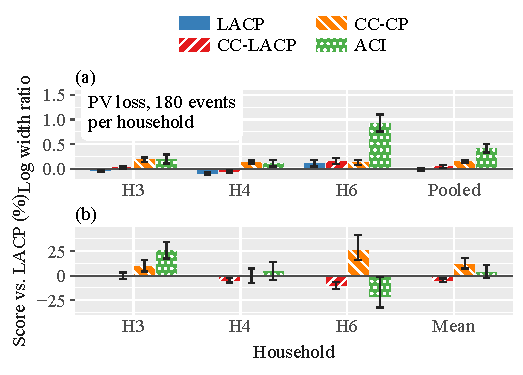
\includegraphics{figures/fig_households.pdf}
\caption{PV loss by household: (a) log width ratio, injected over control window, (b) in-event score against
LACP.}
\label{fig:households}
\end{minipage}\hfill
\begin{minipage}[t]{252pt}\centering
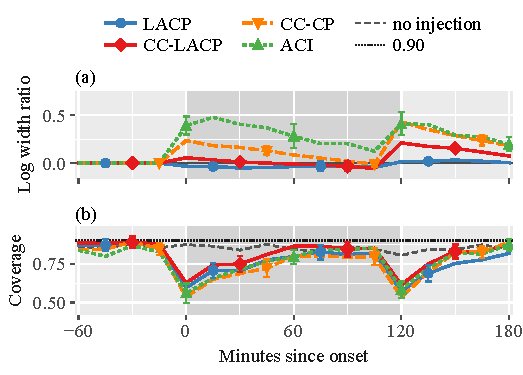
\includegraphics{figures/fig_eventtime.pdf}
\caption{Through a 120-min PV loss (shaded): (a) log width ratio by issue time, (b) coverage by target time.
Error bars at staggered times.}
\label{fig:eventtime}
\end{minipage}
\end{figure*}

\subsection{Q1: Learned Difficulty Scale under PV Loss}
\emph{Fig.~\ref{fig:households}---PV loss by household:} LACP narrows under PV loss in H3 and H4, widens in H6,
and is narrower than in the control window in \narrowLACP{} of all PV-loss windows. The consistency factor widens
LACP in every household. CC-LACP scores lower than LACP under PV loss in H4 and H6 and not distinguishably in H3,
and ACI widens most in H6.

\emph{Fig.~\ref{fig:eventtime}---Interval through a loss:} The first disturbed targets are forecast before the
onset, and every method covers only \covOnsetMin{} to \covOnsetMax{} of them. ACI widens most from the first
disturbed issue time, as its first update uses the uncovered target at the onset, and stays wide until the loss
ends. The CC-CP widening peaks at the onset and fades as the normal-behaviour models follow the new PV level, and
LACP stays narrower than in the control window. In the first hour CC-LACP covers \covHourCCLACP{} of the targets,
\covHourDCCLACPvsLACP{} \covHourDCCLACPvsLACPCI{} more than LACP and \covHourDCCLACPvsACI{}
\covHourDCCLACPvsACICI{} more than ACI.

\emph{Fig.~\ref{fig:severity}---Depth of the loss:} The LACP width ratio falls as the loss deepens and drops below
one at $s=0.75$. The width added by the factor grows with the loss, so the CC-LACP ratio stays level, while the
CC-CP and ACI ratios rise.

\subsection{Q2: Accuracy with the Consistency Factor}
\begin{figure*}[t]
\centering
\begin{minipage}[t]{252pt}\centering
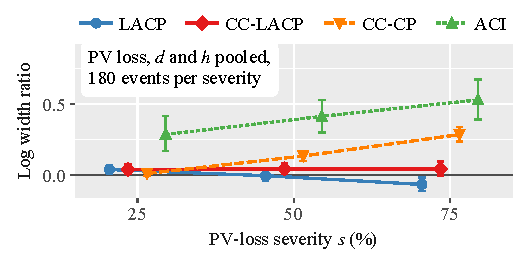
\includegraphics{figures/fig_severity.pdf}
\caption{Log width ratio under PV loss against the loss severity.}
\label{fig:severity}
\end{minipage}\hfill
\begin{minipage}[t]{252pt}\centering
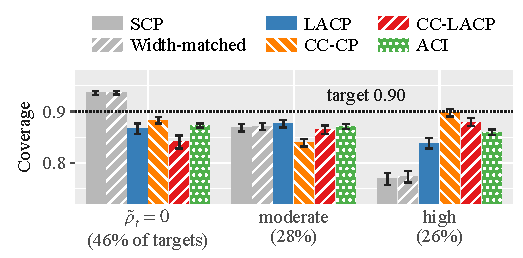
\includegraphics{figures/fig_bands.pdf}
\caption{Normal-operation coverage by consistency band. Width-matched: SCP at the mean width of CC-CP.}
\label{fig:bands}
\end{minipage}
\end{figure*}

\emph{Table~\ref{tab:results}---Static calibration:} In normal operation CC-LACP changes the LACP score by
\cleanrelCCLACP, with counts \dmCCLACPvsLACP. Inside disturbances it changes it by
\relCCLACPvsLACP{} \relCCLACPvsLACPCI, from \relCCLACPvsLACPHSix{} in H6 to \relCCLACPvsLACPHThree{} in H3, and the
recovery-target score by \recrelCCLACP. CC-LACP scores \relCCLACPvsWM{} \relCCLACPvsWMCI{} against
the width-matched control, which knows the event window, so the gain lies in how much width the factor adds. On the held-out complete trips it
changes the LACP score by \triprelCCLACP{} \triprelCCLACPCI{} and raises coverage from \tripLACPPICP{} to
\tripCCLACPPICP. The 3.7-kW steps fall outside most intervals, and the factor lowers their LACP score by
\evabsCCLACP, against \evabsACI{} for ACI.

\emph{Where the factor lowers the score:} The factor trades width for misses. Over the \nCells{} event cells (household, type,
severity, duration, horizon), its change of the LACP in-event score rises with the in-event
coverage of LACP (rank correlation \cellRho, \cellRhoDev{} on development events). It runs from \binLow{}
\binLowCI{} where LACP covers less than 0.75 of the disturbed targets to \binHigh{} \binHighCI{} where it covers 0.90 or more,
and the fitted change is zero near \cellCross. LACP covers \covLACPinHThree{} of the in-event targets in H3,
\covLACPinHFour{} in H4 and \covLACPinHSix{} in H6, so in H3 the added width (\dWidthHThree{} of the LACP score)
outweighs the misses removed (\dPenHThree). There the change is \relHThreePV{} under PV loss and \relHThreeLoad{}
and \relHThreeComb{} under load steps and combined events.

\emph{Fig.~\ref{fig:bands}---Normal operation by consistency score:} With bands at zero and at the calibration
median of the positive scores, SCP covers \bandZeroSCP{} of the targets at zero score and \bandHighSCP{} in the
high band, so the score marks periods of larger forecast error. CC-CP and CC-LACP raise high-band coverage to
\bandHighCCCP{} and \bandHighCCLACP, and a fixed interval with the mean width of CC-CP reaches \bandHighWMS, so the
gain comes from where the width is placed. CC-LACP covers less than LACP at zero score.

\begin{figure*}[t]
\centering
\begin{minipage}[t]{252pt}\centering
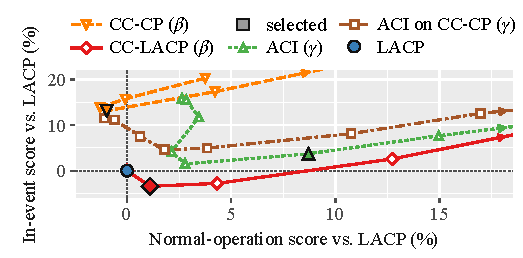
\includegraphics{figures/fig_tradeoff.pdf}
\caption{Gain and step sweeps, from the smallest value to the arrow (off range: $\gamma=0.5$, CC-CP $\beta=4$,
CC-LACP $\beta=2$).}
\label{fig:tradeoff}
\end{minipage}\hfill
\begin{minipage}[t]{252pt}\centering
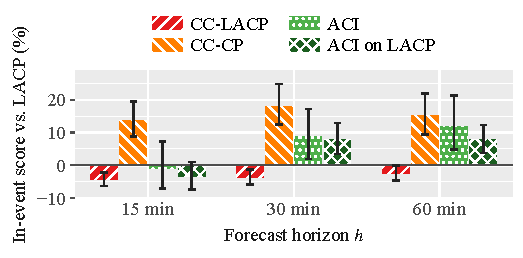
\includegraphics{figures/fig_horizon.pdf}
\caption{In-event score against LACP by horizon, 120-min events, first 45~min.}
\label{fig:horizon}
\end{minipage}
\end{figure*}

\emph{Fig.~\ref{fig:tradeoff}---Gains and steps:} Only CC-LACP with the selected gain scores below LACP inside
events with a normal-operation score within 2\%, and larger gains raise both scores. ACI stays above LACP inside
events at every step, and CC-CP at least 13\% above it for every gain. The factor lowers both scores of ACI at the
smallest steps and raises both at the selected step, where the rule sets its gain to zero.

\begin{table}[t]
\caption{Variants of the consistency signal, gains selected by the same rule. Net adaptation to injected PV
loss and load steps and in-event score against LACP. $^{*}$95\% interval excludes zero.}
\label{tab:ablation}
\centering
\scriptsize
\setlength{\tabcolsep}{2.4pt}
\renewcommand{\arraystretch}{0.90}\begin{tabular}{|l|c|c|c|c|}
\hline
\multirow{2}{*}{Signal} & \multirow{2}{*}{$\beta$} & \multicolumn{2}{c|}{Net adaptation} & Score vs.\\
\cline{3-4}
 & & PV loss & Load step & LACP\\
\hline
\multicolumn{5}{|l|}{\emph{Scale $1+\beta\tilde\rho_t$ (CC-CP)}}\\
\quad None (SCP) & -- & +0.000 & +0.000 & +20.3\%\\
\quad PV and load & 1 & +0.192$^{*}$ & +0.090$^{*}$ & +13.2\%\\
\quad PV only & 1 & +0.285$^{*}$ & +0.000 & +12.6\%\\
\quad Load only & 0.25 & +0.000 & +0.022$^{*}$ & +17.6\%\\
\quad Load model, day lag only & 1 & +0.210$^{*}$ & +0.063$^{*}$ & +11.4\%\\
\quad Both, day lag only & 0.25 & $-$0.010 & +0.056$^{*}$ & +17.2\%\\
\quad Persistence residual & 1 & +0.133$^{*}$ & +0.059$^{*}$ & +17.1\%\\
\hline
\multicolumn{5}{|l|}{\emph{Scale $s(x_t)(1+\beta\tilde\rho_t)$ (CC-LACP)}}\\
\quad None (LACP) & -- & $-$0.021$^{*}$ & +0.114$^{*}$ & 0\\
\quad PV and load & 0.25 & +0.039$^{*}$ & +0.114$^{*}$ & $-$3.4\%\\
\quad PV only & 0.25 & +0.045$^{*}$ & +0.107$^{*}$ & $-$3.5\%\\
\quad Persistence residual & 0.25 & +0.011 & +0.110$^{*}$ & $-$0.9\%\\
\quad Indicator $\mathbf{1}\{\tilde\rho_t>\tau\}$ & 0.5, $\tau=q_{80}$ & +0.033$^{*}$ & +0.122$^{*}$ & $-$2.7\%\\
\hline
\end{tabular}

\end{table}

\emph{Table~\ref{tab:ablation}---Signal design:} With the constant base, the PV channel carries the response to
PV loss and the load channel the response to load steps, so the maximum in \eqref{eq:rho} retains both. Models
that see only the day-lag value and the calendar lose the PV-loss response, and a persistence residual responds
less and scores worse. On the LACP scale $s(x_t)$ carries the load-step response, the PV channel alone gives
nearly the gain of both, and the persistence residual and the indicator give less.

\subsection{Q3: Error-Driven Recalibration}
\emph{Table~\ref{tab:results}---Rolling and adaptive calibration:} Against ACI with $\gamma=\selACI$, CC-LACP
changes the in-event score not distinguishably, by \relCCLACPvsACI{} \relCCLACPvsACICI, with opposite signs by
household, and has normal-operation counts \dmCCLACPvsACI. ACI covers more inside disturbances (\inACIPICP{} against
\inCCLACPPICP) at a normal-operation score \abscleanrelACI{} above LACP, and the clip in \eqref{eq:aci} holds its
normal-operation coverage at \cleanACIPICP{} (\unclipPICP{} unclipped, at a higher score). Inside disturbances
CC-LACP scores \absrelCCLACPvsACIL{} below ACI on LACP and \absrelCCLACPvsROLLLACP{} below rolling LACP.
Recalibrating on recent scores lifts normal-operation coverage from \cleanStaticMin--\cleanStaticMax{} (static,
lowered by drift) to about 0.90 and leaves the factor no significant in-event gain
(\relROLLCCLACPvsROLLLACP{} \relROLLCCLACPvsROLLLACPCI{} in the rolling window, \relACICCLvsACIL{}
\relACICCLvsACILCI{} in ACI on LACP). In both, the factor still widens the interval at the onset of a 120-min loss,
raises first-hour coverage by \covHourFROLL{} and \covHourFACIL, and changes the 3.7-kW-step score by \evfacROLL{}
and \evfacACIL. The net PV-loss adaptation of CC-CP and ACI is not distinguishable, and without injection the width
exceeds 1.25 times its pre-event median in \faLACP, \faCCLACP{} and \faACI{} of LACP, CC-LACP and ACI windows.

\emph{Fig.~\ref{fig:horizon}---Forecast horizon:} CC-LACP stays below LACP at every horizon,
while ACI moves from \hzACIShort{} at 15~min to \hzACILong{} at 60~min and ACI on LACP from \hzACILShort{} to
\hzACILLong, consistent with feedback that arrives $h$ steps late.

\subsection{Q4: Battery Reserve}
\begin{table}[t]
\caption{Battery reserve at the 15-min horizon: reserve adequacy, shortfall (uncovered next-step energy) and
grid import (kWh per event). Bold: best interval reserve.}
\label{tab:battery}
\centering
\scriptsize
\setlength{\tabcolsep}{2pt}
\renewcommand{\arraystretch}{0.95}\begin{tabular}{|l|c|c|c|c|c|c|c|}
\hline
\multirow{2}{*}{Reserve from} & \multicolumn{4}{c|}{Adequacy, injected window} & \multirow{2}{*}{\hdb{Short-\\fall}} & \multirow{2}{*}{\hdb{Grid\\import}} & \multirow{2}{*}{\hdb{Adequacy,\\control}}\\
\cline{2-5}
 & \hdb{PV\\loss} & \hdb{Load\\step} & \hdb{PV\\trip} & All & & & \\
\hline
No battery & -- & -- & -- & -- & -- & 0.843 & --\\
Point only & 0.770 & 0.549 & 0.751 & 0.688 & 0.295 & 0.594 & 0.810\\
SCP & 0.851 & \textbf{0.788} & 0.805 & 0.818 & 0.153 & \textbf{0.604} & 0.942\\
LACP & 0.866 & 0.700 & 0.822 & 0.800 & 0.154 & 0.611 & 0.924\\
CC-CP & 0.851 & 0.750 & 0.809 & 0.806 & 0.160 & 0.607 & 0.934\\
\rowcolor{black!6}
CC-LACP & 0.871 & 0.692 & 0.831 & 0.801 & 0.154 & 0.613 & 0.921\\
Rolling LACP & 0.883 & 0.743 & 0.846 & 0.827 & 0.125 & 0.613 & \textbf{0.947}\\
Rolling CC-LACP & 0.889 & 0.735 & 0.850 & 0.828 & 0.122 & 0.616 & 0.945\\
ACI & 0.871 & 0.775 & 0.836 & 0.827 & 0.136 & 0.611 & 0.942\\
ACI on LACP & 0.888 & 0.755 & 0.847 & \textbf{0.832} & 0.121 & 0.614 & 0.945\\
ACI on CC-LACP & \textbf{0.893} & 0.742 & \textbf{0.863} & 0.831 & \textbf{0.119} & 0.616 & 0.946\\
\hline
\end{tabular}

\end{table}

\emph{Table~\ref{tab:battery}---Reserve adequacy:} Every interval reserve covers the next-step demand in
\batAdqIntMin{} to \batAdqIntMax{} of the disturbed steps, against \batAdqPoint{} for the point reserve, with at
most \batImpRise{} more grid import. The rolling and ACI reserves on the LACP and CC-LACP scores have the highest
adequacy under PV loss and trips. The factor raises the LACP adequacy under PV loss and trips by less than 0.01 and
the ACI-on-LACP adequacy under trips by \batTripAdqACICCLvsACILAbs, and lowers the load-step adequacy slightly on
all three bases. Under load steps SCP and ACI rank highest.

\subsection{Robustness and Limitations}
CC-LACP changes the LACP in-event score by \robclipCCLACPvsLACP{} \robclipCCLACPvsLACPCI{} with load clipped at
zero, by \robmlpCCLACPvsLACP{} \robmlpCCLACPvsLACPCI{} with the neural backbone and by \robfrzCCLACPvsLACP{}
\robfrzCCLACPvsLACPCI{} on a second, independent set of two onsets per configuration and household (\nFrozen{} of 162, one follows a
data gap). The limitations and how they are
addressed are:
\begin{itemize}
\item \emph{Simulated disturbances.} No inverter status is recorded, so disturbances are injected through the
same models as the record and compared with their control windows. Held-out trips and 3.7-kW steps test larger
events.
\item \emph{Three households.} Results are reported per household with intervals over household-days. Selected on
two households and tested on the third, the gain changes the score by \lohorelHThree, \lohorelHFour{} and
\lohorelHSix{} in H3, H4 and H6.
\item \emph{Household dependence.} Where the unmodified interval already covers the disturbance, as in most H3
events, the factor raises the score. Selection per household on development data sets the gain to zero in H3,
where it lowers neither score, and in H6, where it raises the normal-operation score beyond the 2\% tolerance.
\item \emph{Serial dependence.} Time series and disturbances violate exchangeability, so coverage is measured and
score differences carry a Newey--West variance.
\item \emph{Lasting losses.} During a lasting loss the score returns to its control level within about 90~min. With
a rolling window or ACI, which follow lasting shifts, the factor still widens the interval at the onset.
\end{itemize}

\section{Conclusion}\label{sec:conclusion}
Conformal intervals for the net load of three households were scaled by a measured consistency score of PV and load and
tested on injected disturbances, held-out trips and load steps, and a battery reserve. A learned difficulty
scale narrows in most PV losses, the more so the deeper the loss. The consistency factor counteracts this
narrowing, lowers the interval score during disturbances and raises first-hour coverage at a slightly higher
normal-operation score, the more so the more of the disturbance the unmodified interval misses. Inside disturbances
it is not distinguishable from fixed-step ACI, whose normal-operation score is higher, and once the quantile follows
recent scores it gives no significant in-event gain. For a battery reserve the calibration method matters more.
Recalibration on recent scores thus comes first, and the factor adds first-hour coverage and a lower score
under large load steps, so that the interval follows a PV loss through a measured departure from normal behaviour
and not only through past forecast errors. Future work will test the score on recorded inverter faults and more
households and combine it with online step tuning.

\bibliographystyle{IEEEtran}
\bibliography{refs}

\end{document}
